\documentclass[conference]{IEEEtran}
\IEEEoverridecommandlockouts
% The preceding line is only needed to identify funding in the first footnote. If that is unneeded, please comment it out.
\usepackage{cite}
\usepackage{amsmath,amssymb,amsfonts}
\usepackage{algorithmic}
\usepackage{graphicx}
\usepackage{textcomp}
\usepackage{xcolor}
\usepackage{booktabs}
\usepackage{tabularx} 
\usepackage{multirow}
\usepackage{caption} 
\usepackage{makecell}
\usepackage{hyperref}
\bibliographystyle{IEEEtran} 
\def\BibTeX{{\rm B\kern-.05em{\sc i\kern-.025em b}\kern-.08em
    T\kern-.1667em\lower.7ex\hbox{E}\kern-.125emX}}
\begin{document}

\title{Supplementary Materials for the InterMoBA}
\maketitle

\begin{figure*}[htbp]
    \centering
    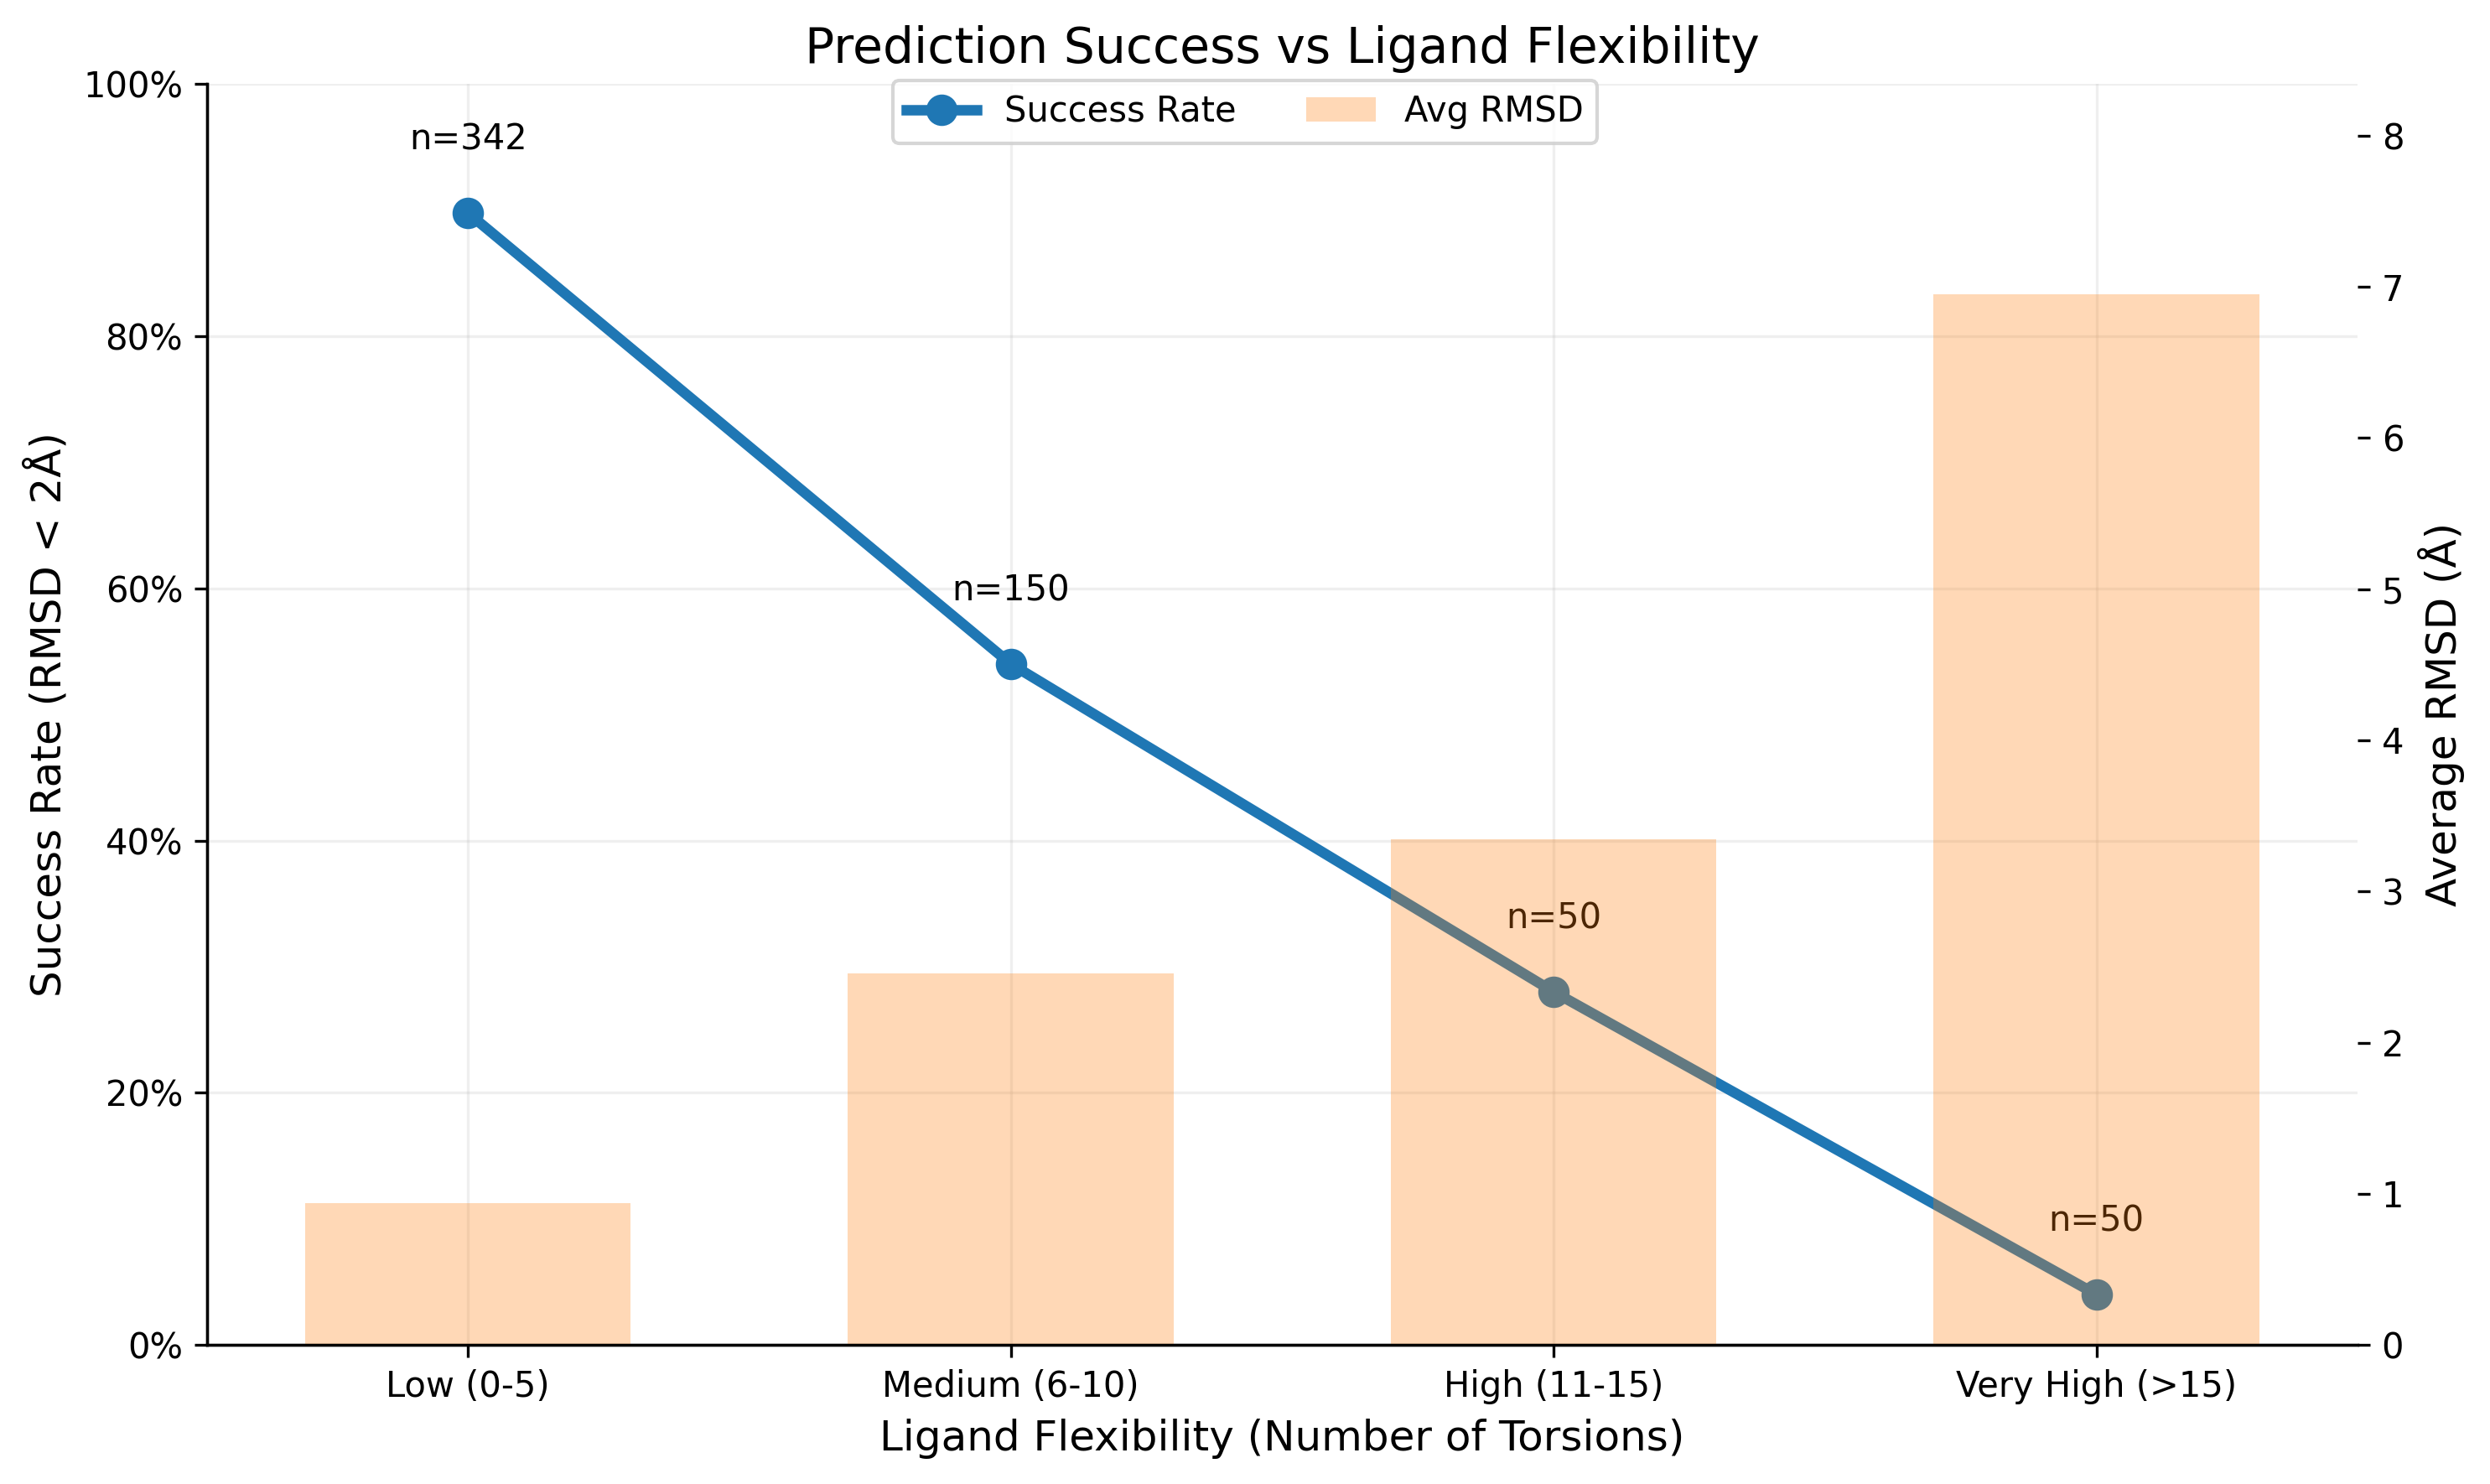
\includegraphics[width=0.8\textwidth]{1.png}  % ← 占全图
    \captionsetup{labelfont=bf,labelsep=space,font=small} % 全局可放导言区
    \caption{\textbf{Correlation analysis between ligand Flexibility and Prediction success rate. Increasing ligand flexibility (rotatable bond count) significantly reduces prediction success (RMSD $<$ 2\AA), from $\sim$90\% (low-flex) to $<$10\% (high-flex), with rising RMSD, highlighting flexibility as a critical accuracy bottleneck.}}
    \label{fig1}


\end{figure*}
 
\begin{figure*}[htbp]
    \centering
    \includegraphics[width=1\textwidth]{2.png} % ← 占全图
    \captionsetup{labelfont=bf,labelsep=space,font=small} % 全局可放导言区
    \caption{
      \textbf{The six sub-diagrams collectively illustrate the effectiveness of the top-ranked poses in comparison to lower-ranked ones across various complexes. Each sub-diagram randomly selects 12 complexes to highlight how the top-ranked poses consistently exhibit lower RMSD values. This consistent trend across all sub-diagrams underscores the model's robustness and its ability to effectively rank poses in practical docking scenarios.
} }
    \label{fig2}
\end{figure*}

 
\begin{figure*}[htbp]
    \centering
    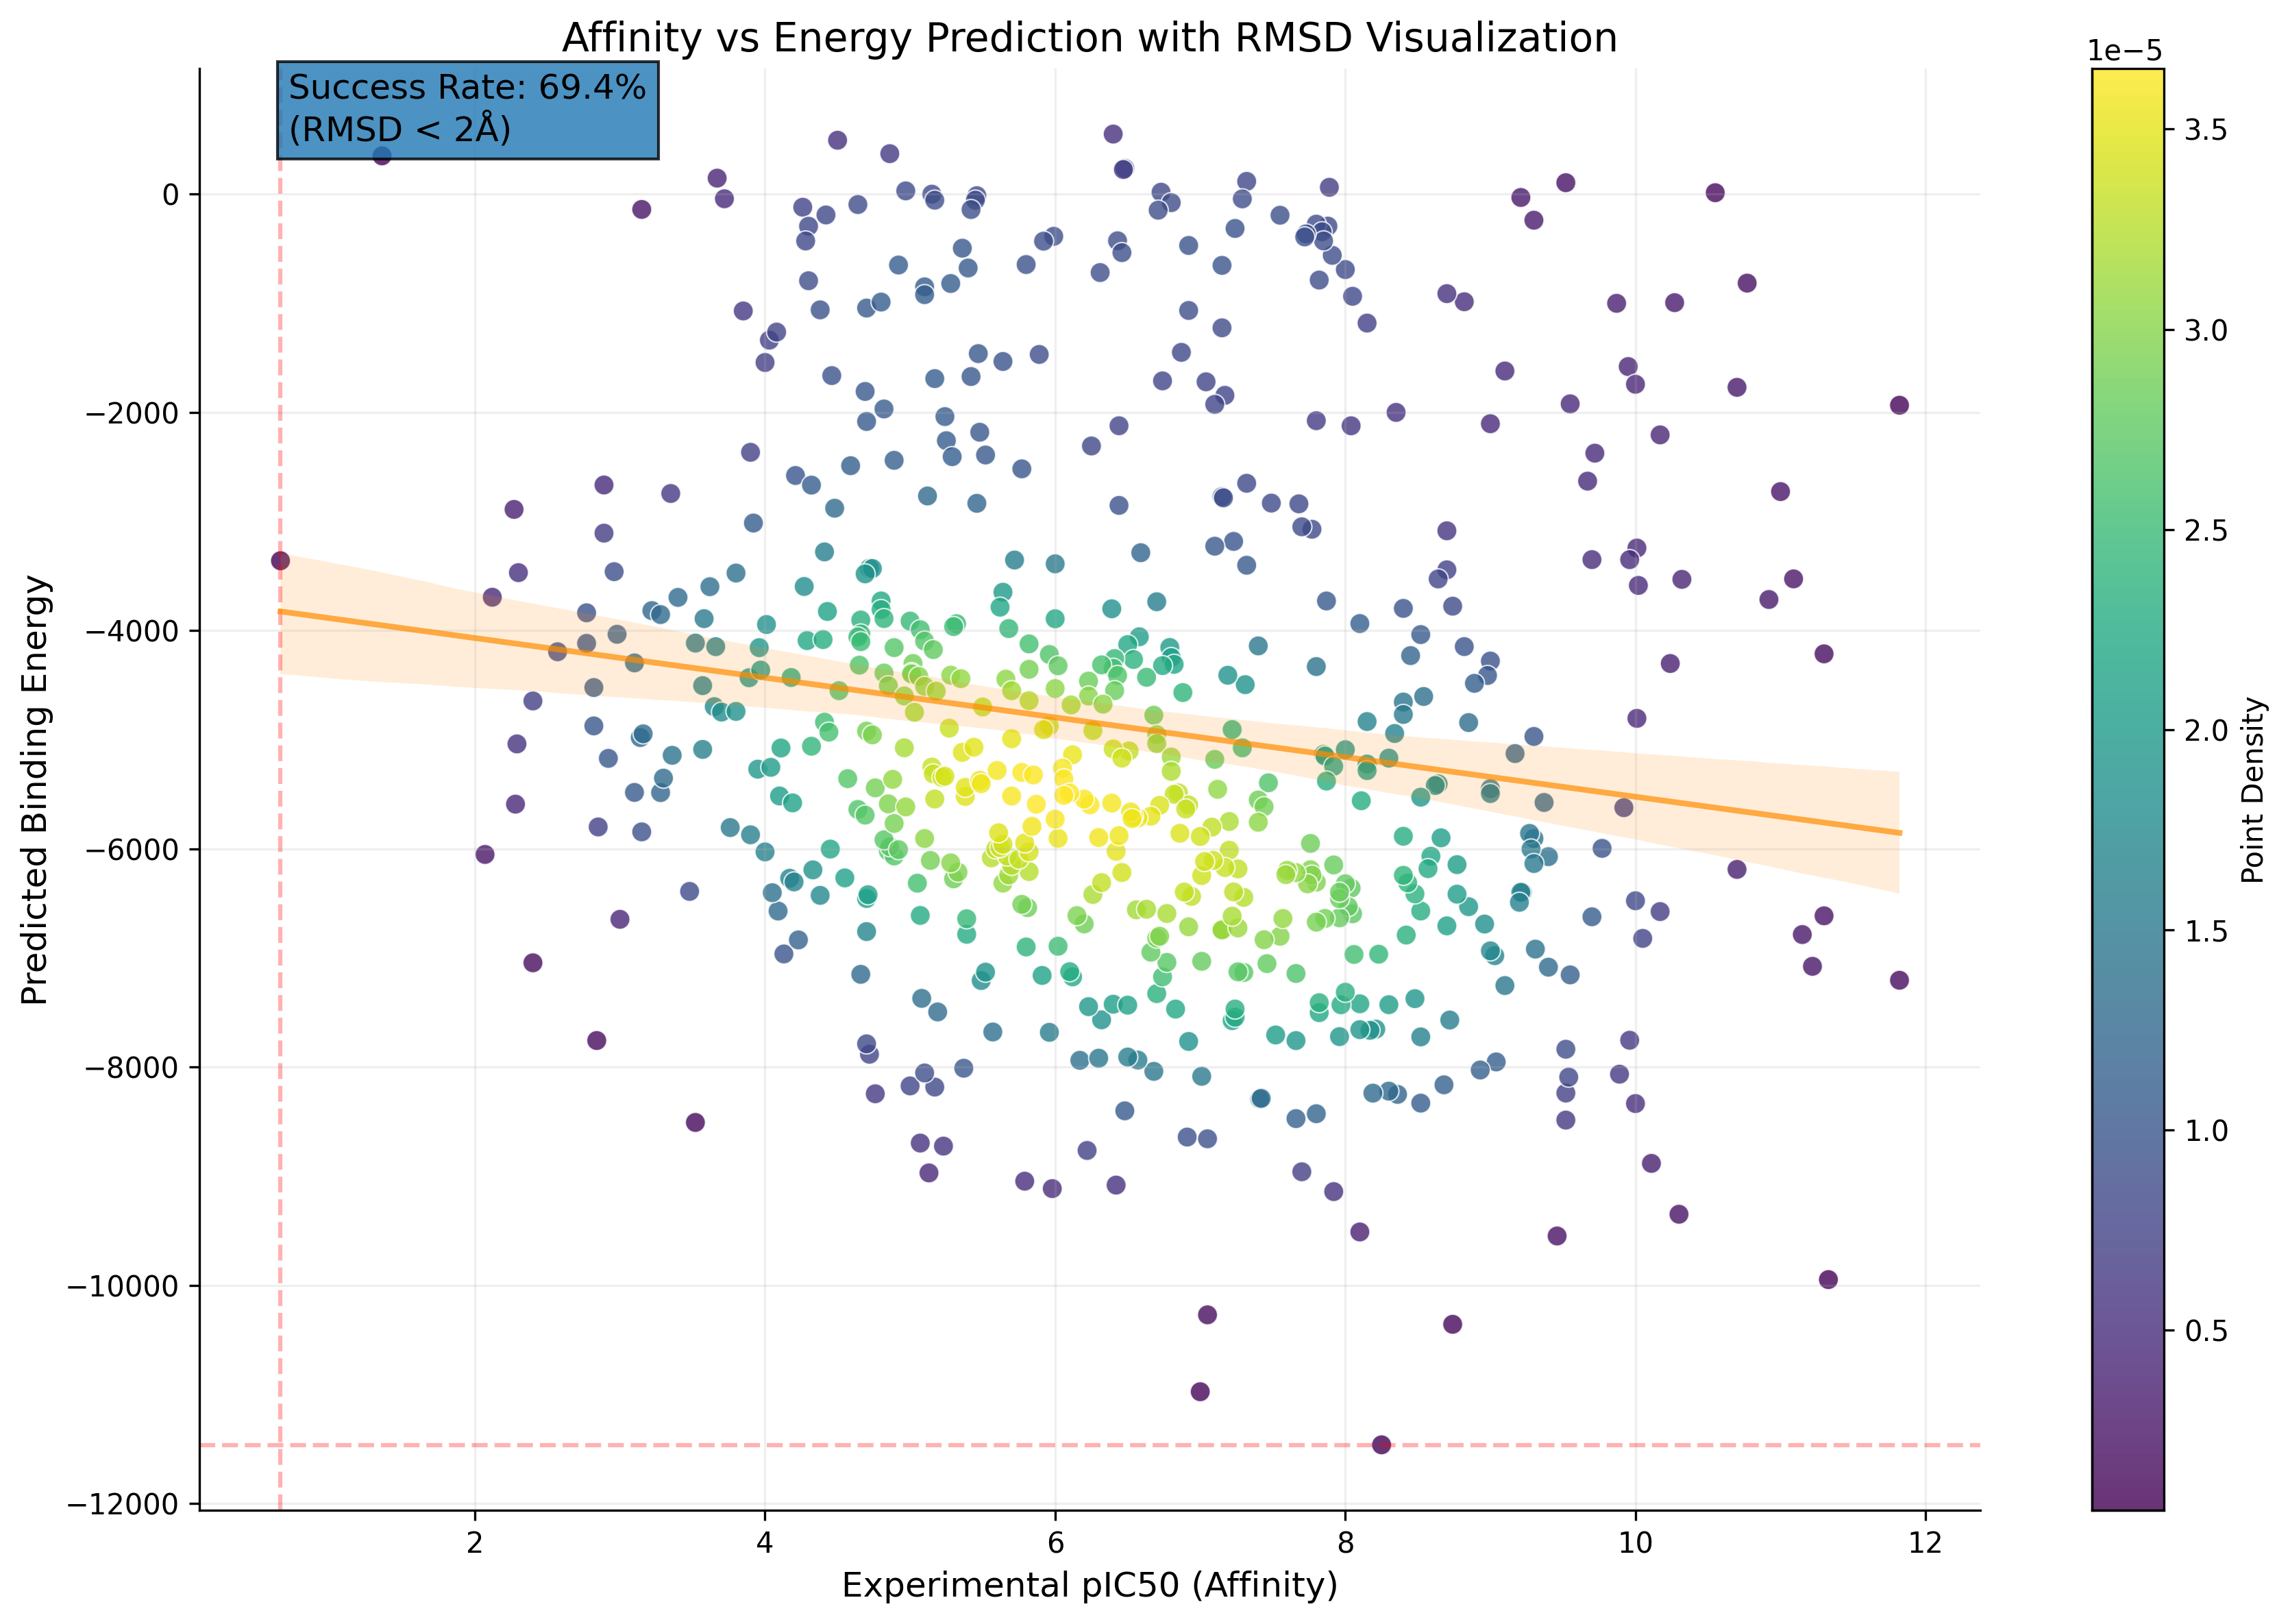
\includegraphics[width=0.8\textwidth]{3.png}  % ← 占全图
    \captionsetup{labelfont=bf,labelsep=space,font=small} % 全局可放导言区
    \caption{
      \textbf{Experimental pIC50 shows a negative correlation with predicted binding energy, demonstrating the model's dual capability in affinity discrimination and conformational prediction.} }
    \label{fig3}
\end{figure*}

 
\begin{figure*}[htbp]
    \centering
    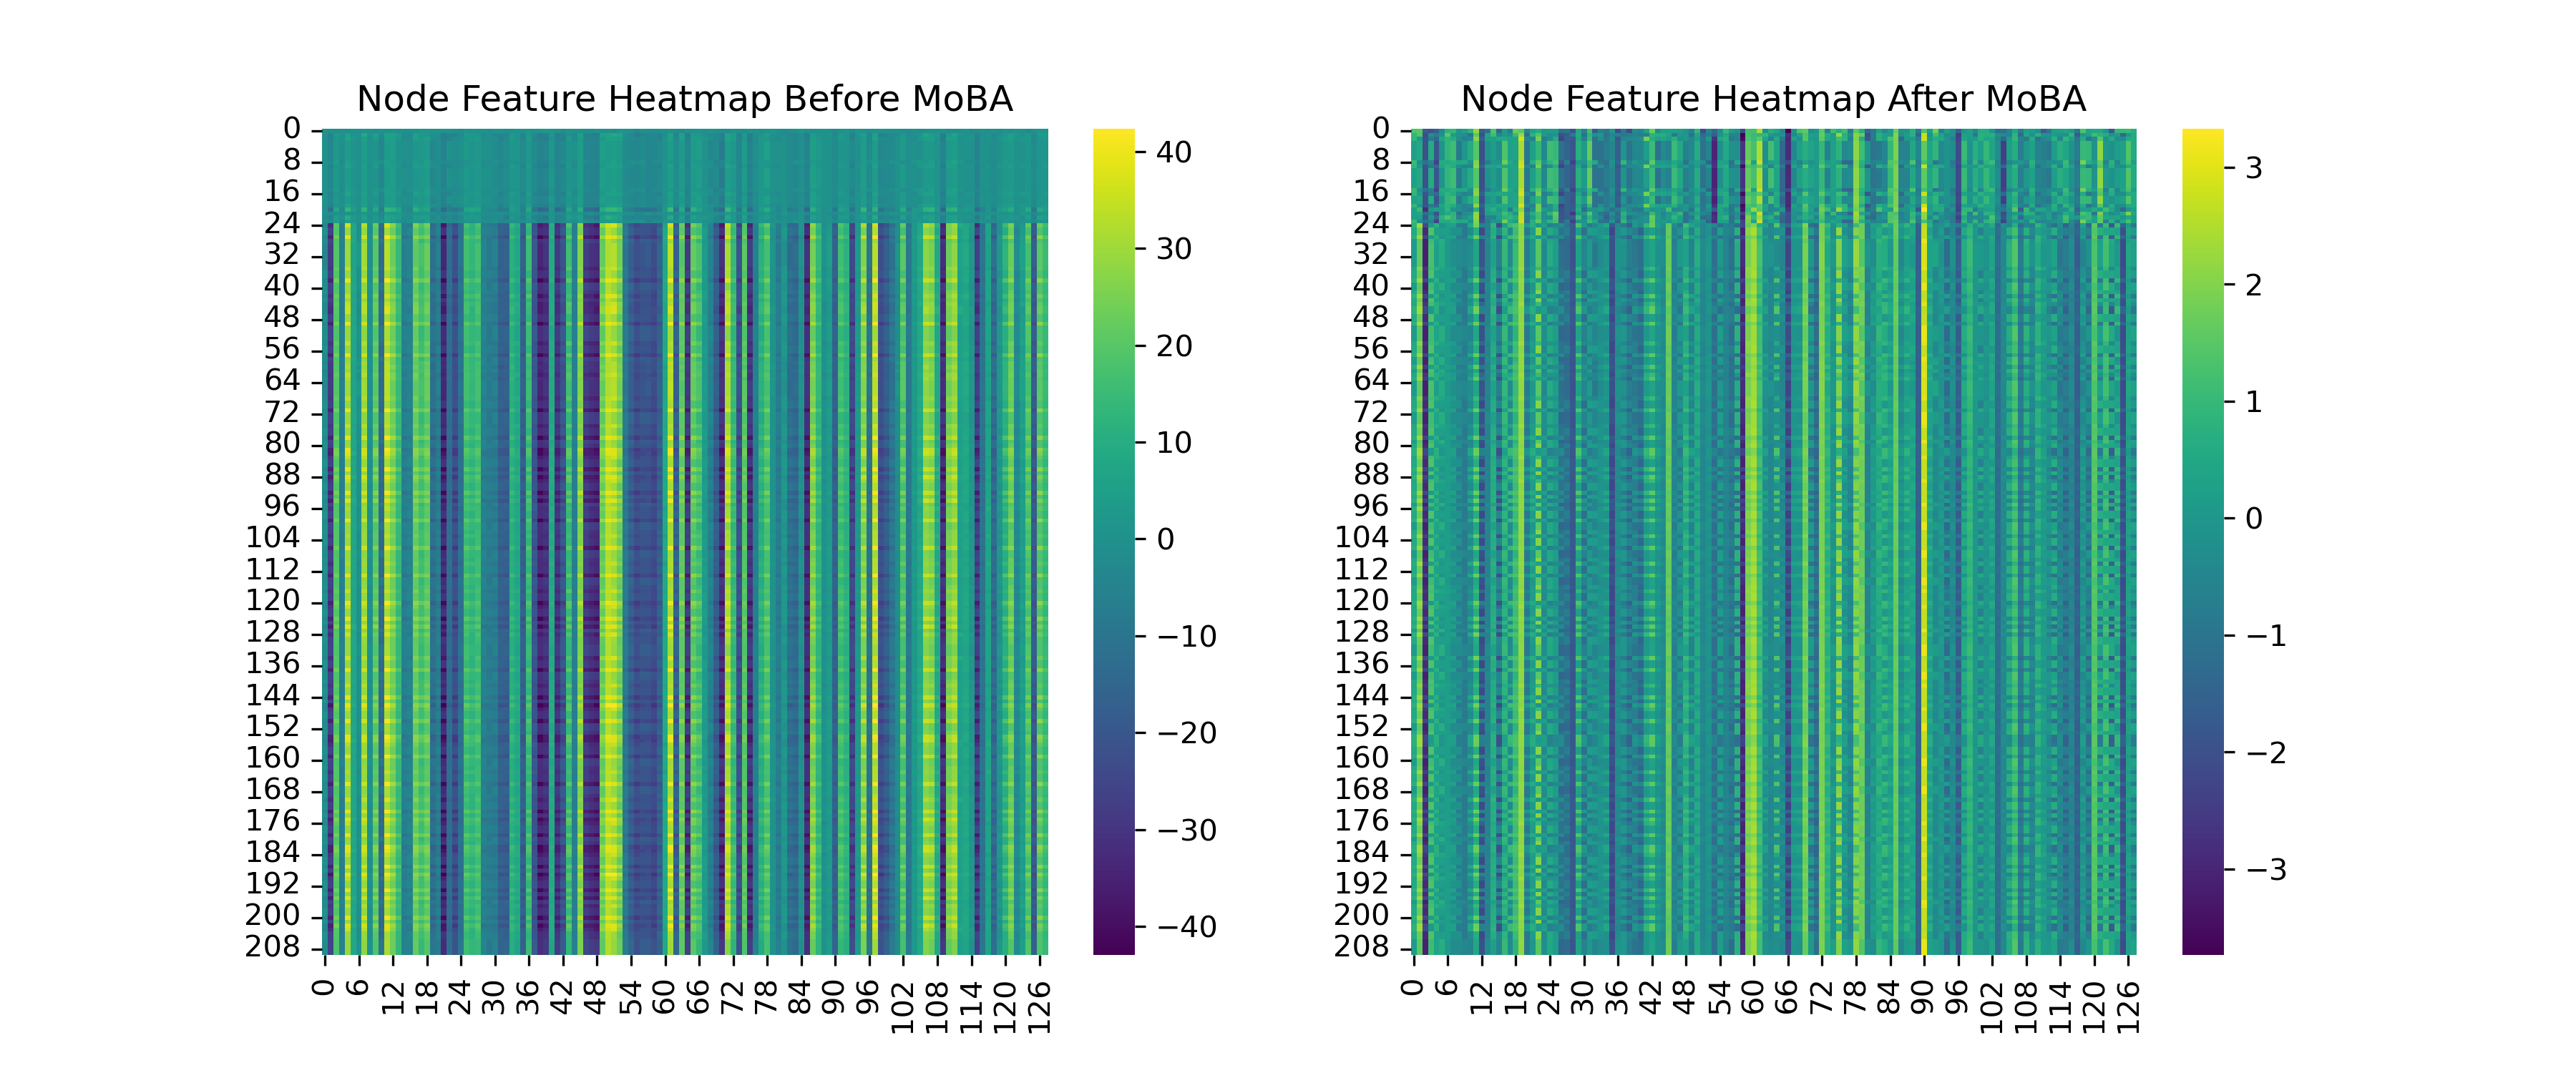
\includegraphics[width=1\textwidth]{4.png}  % ← 占全图
    \captionsetup{labelfont=bf,labelsep=space,font=small} % 全局可放导言区
    \caption{
      \textbf{The MoBA operation significantly alters the distribution of node features, making the feature values more concentrated and evenly distributed, indicating effective normalization and adjustment after MoBA.} }
    \label{fig4}
\end{figure*}

 
\begin{figure*}[htbp]
    \centering
    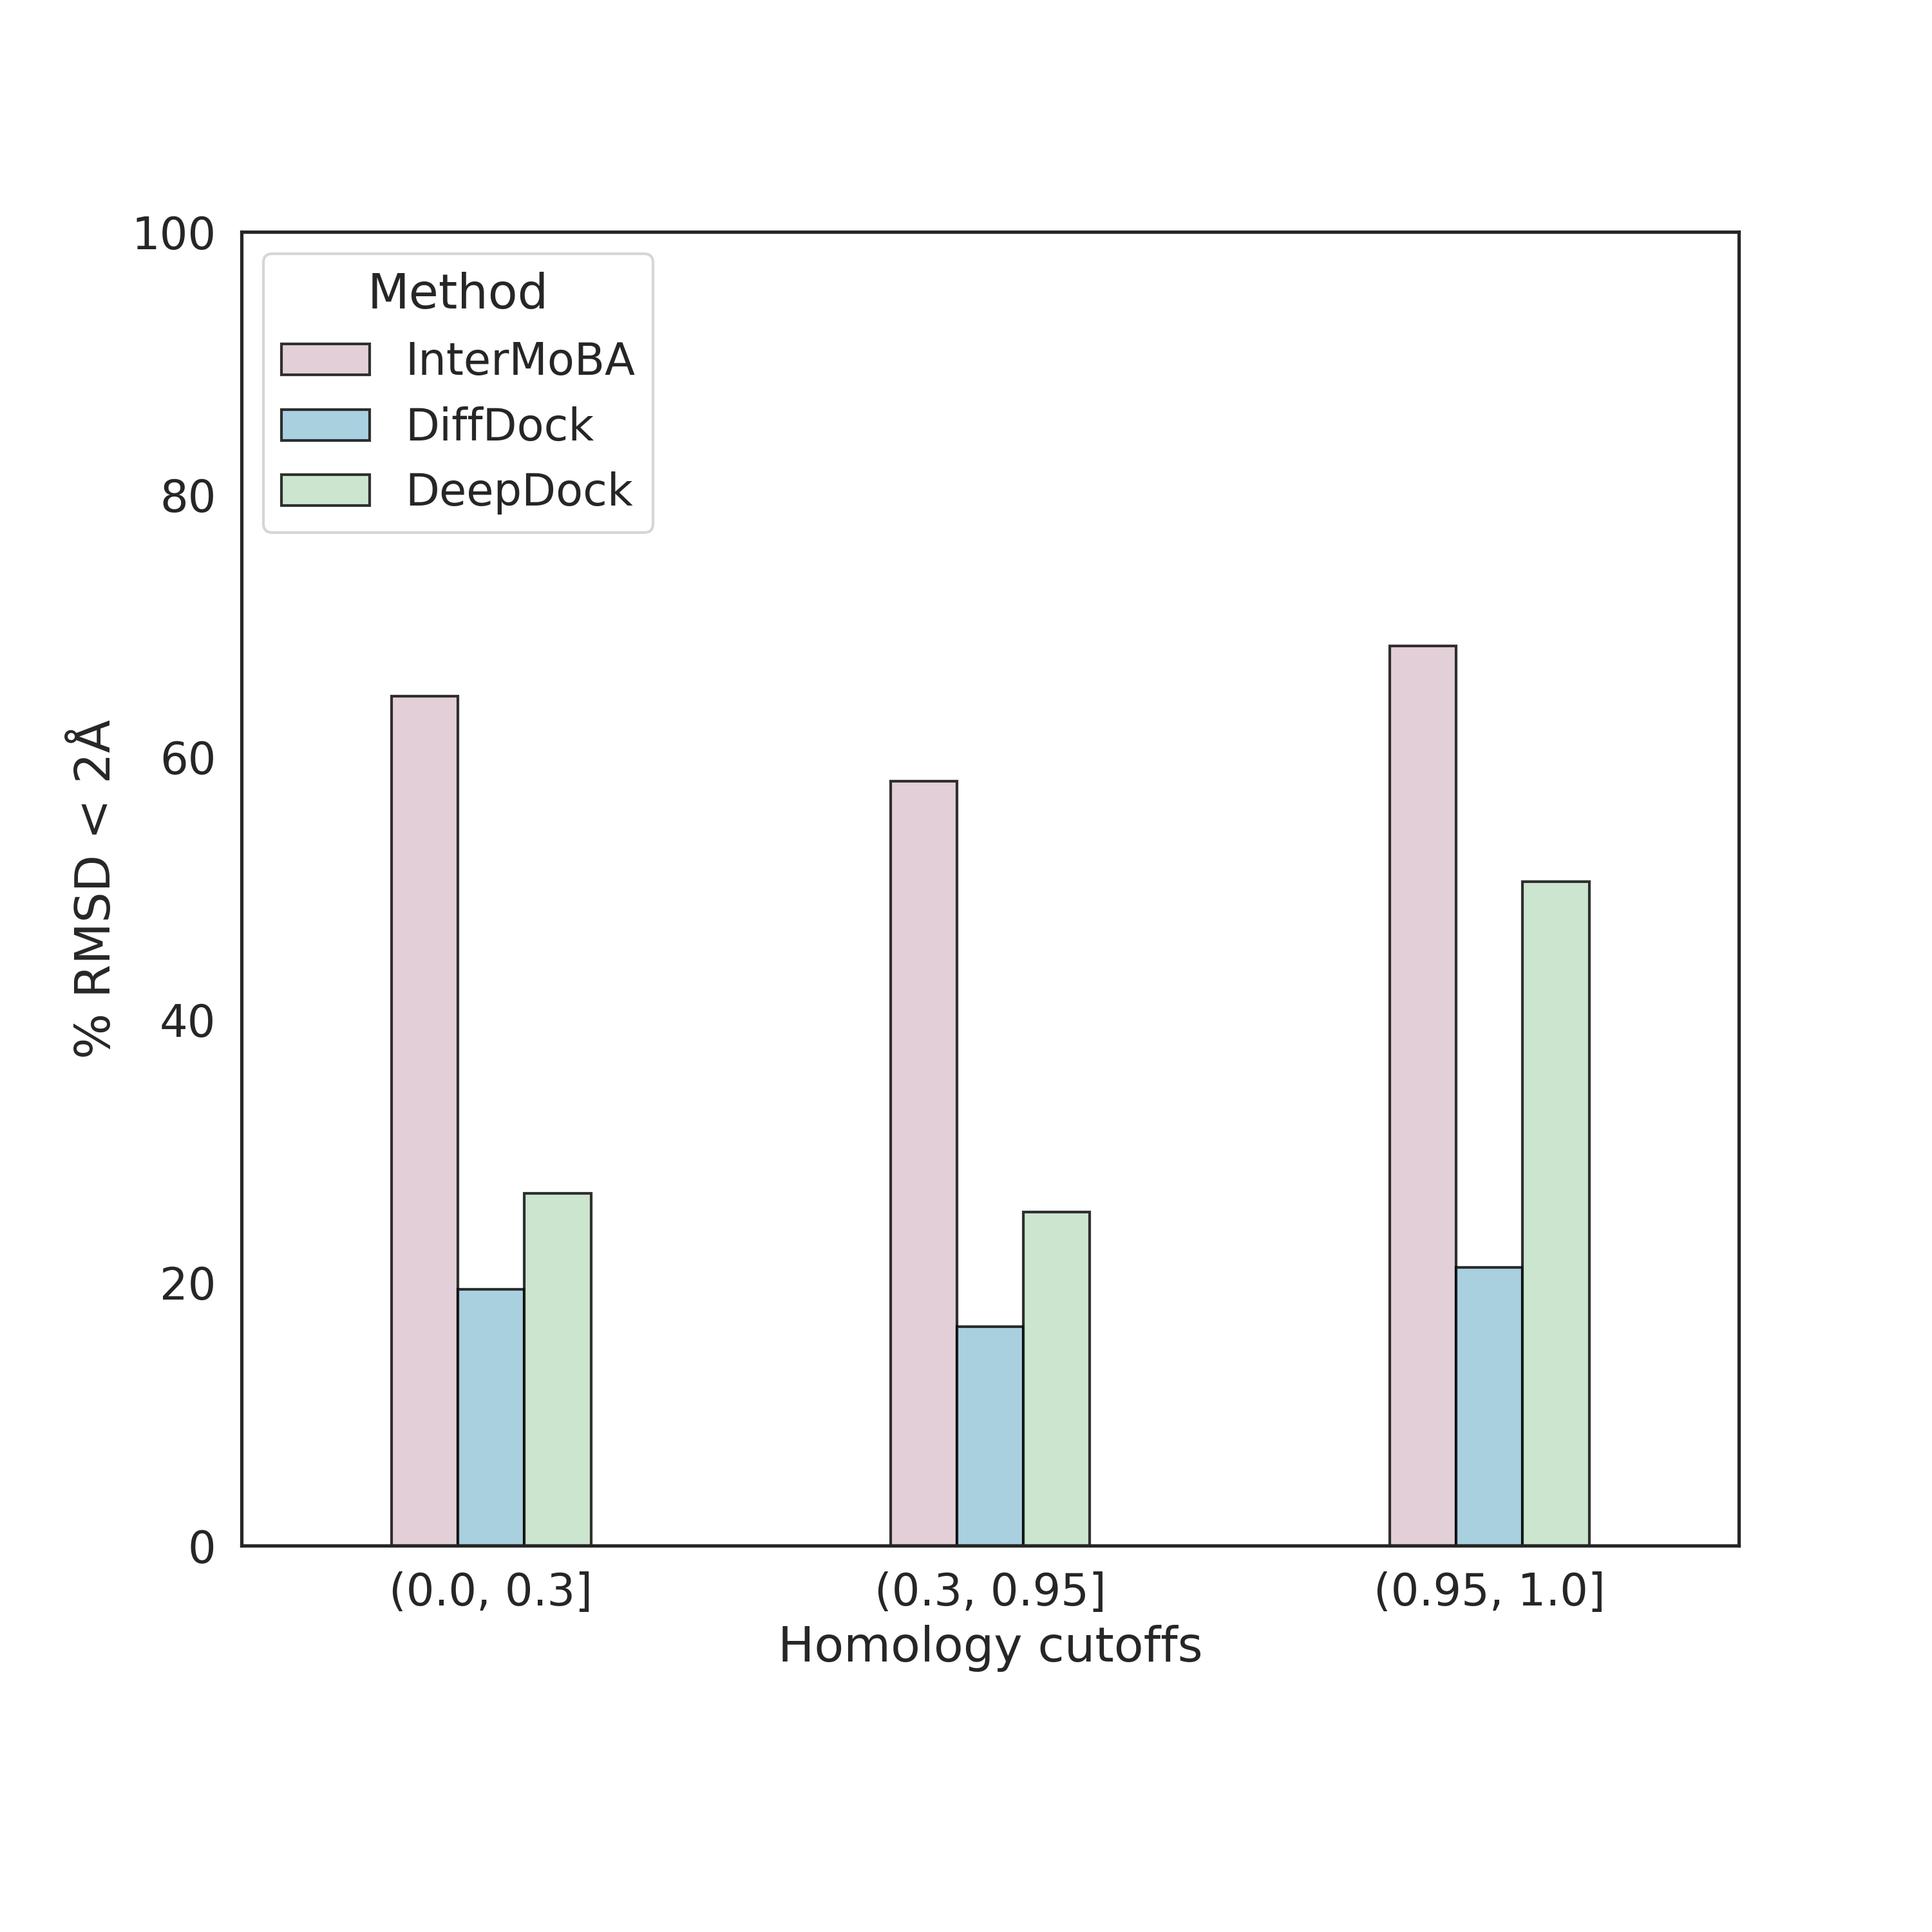
\includegraphics[width=0.9\textwidth]{5.png}  % ← 占全图
    \captionsetup{labelfont=bf,labelsep=space,font=small} % 全局可放导言区
    \caption{
      \textbf{This Figure compares the docking accuracy of three methods—InterMoBA, DiffDock, and DeepDock—across three homology subsets: low (0.0-0.3), medium (0.3-0.95), and high (0.95-1.0). The accuracy is measured as the percentage of poses with RMSD $<$ 2Å. InterMoBA consistently outperforms the other two methods across all homology levels, while DiffDock generally shows the lowest accuracy.} }
    \label{fig5}
\end{figure*}

 
\begin{figure*}[htbp]
    \centering
    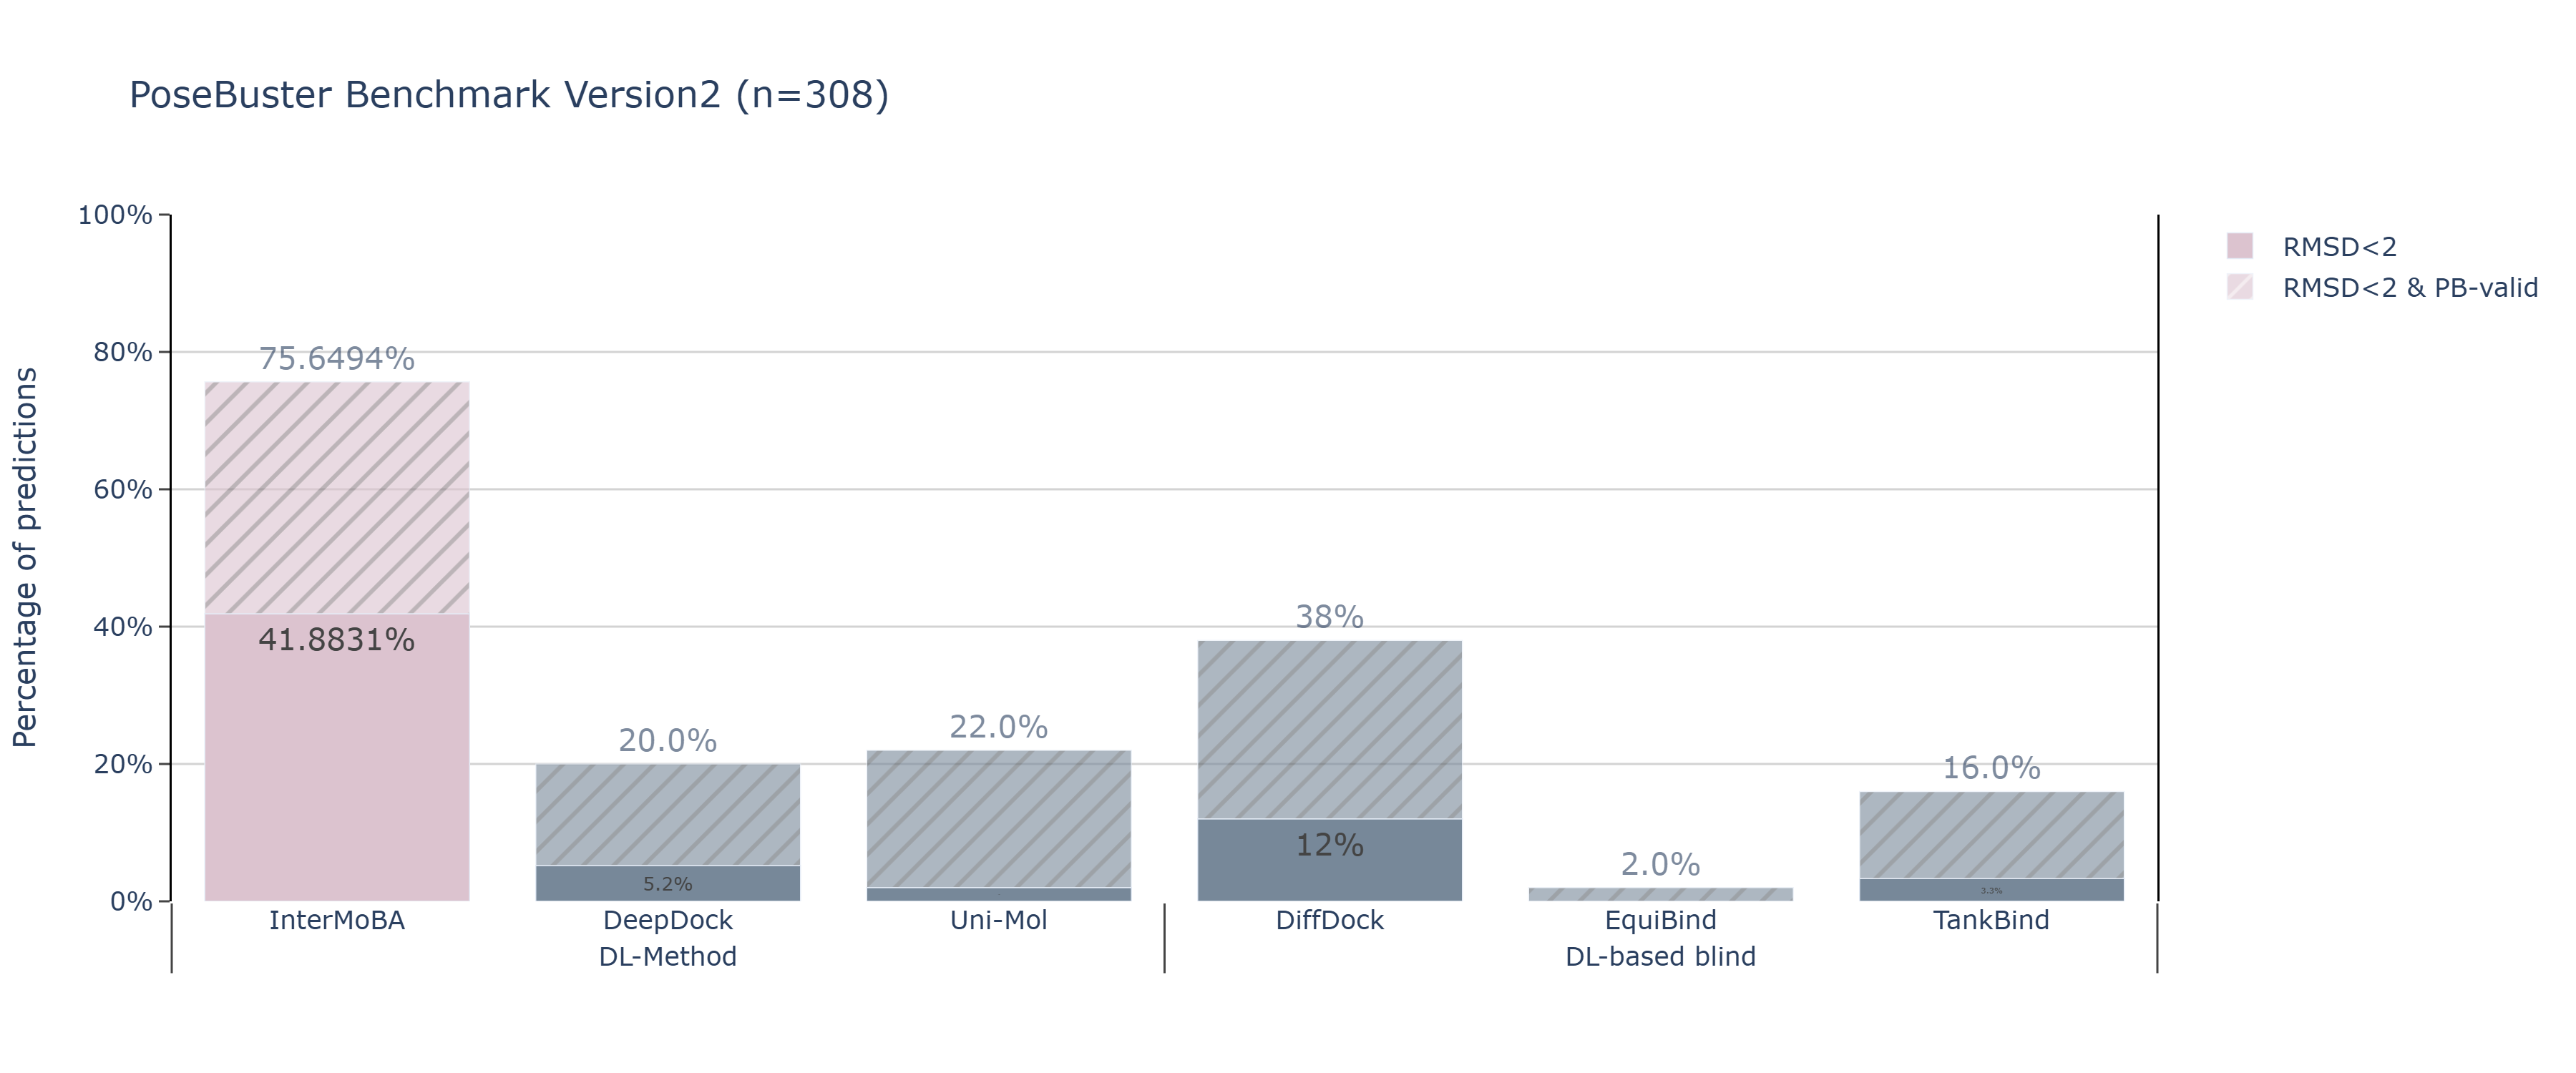
\includegraphics[width=1\textwidth]{6.png}  % ← 占全图
    \captionsetup{labelfont=bf,labelsep=space,font=small} % 全局可放导言区
    \caption{
      \textbf{The figure presents a comparison of success rates among different docking methods on the PoseBusters Benchmark Version 2.}
      \textbf{}The PoseBusters benchmark evaluates molecular docking methods based on their ability to generate physically plausible docking poses, ensuring they meet criteria such as RMSD being less than 2 Å and passing physical plausibility (PB-valid) verification. The figure compares various methods, including deep learning-based approaches such as InterMoBA, DeepDock, Uni-Mol, DiffDock, EquiBind, and TankBind. Each method's bar is divided into two parts: the dark section represents the percentage of predictions with RMSD less than 2 Å, and the light section indicates the percentage that fulfill both RMSD criteria and PoseBusters verification. Furthermore, our model InterMoBA has shown some areas for improvement in the PoseBusters validity check, primarily attributable to issues with atomic distances that necessitate further refinement.} 
    \label{fig6}
\end{figure*}

 
\begin{figure*}[htbp]
    \centering
    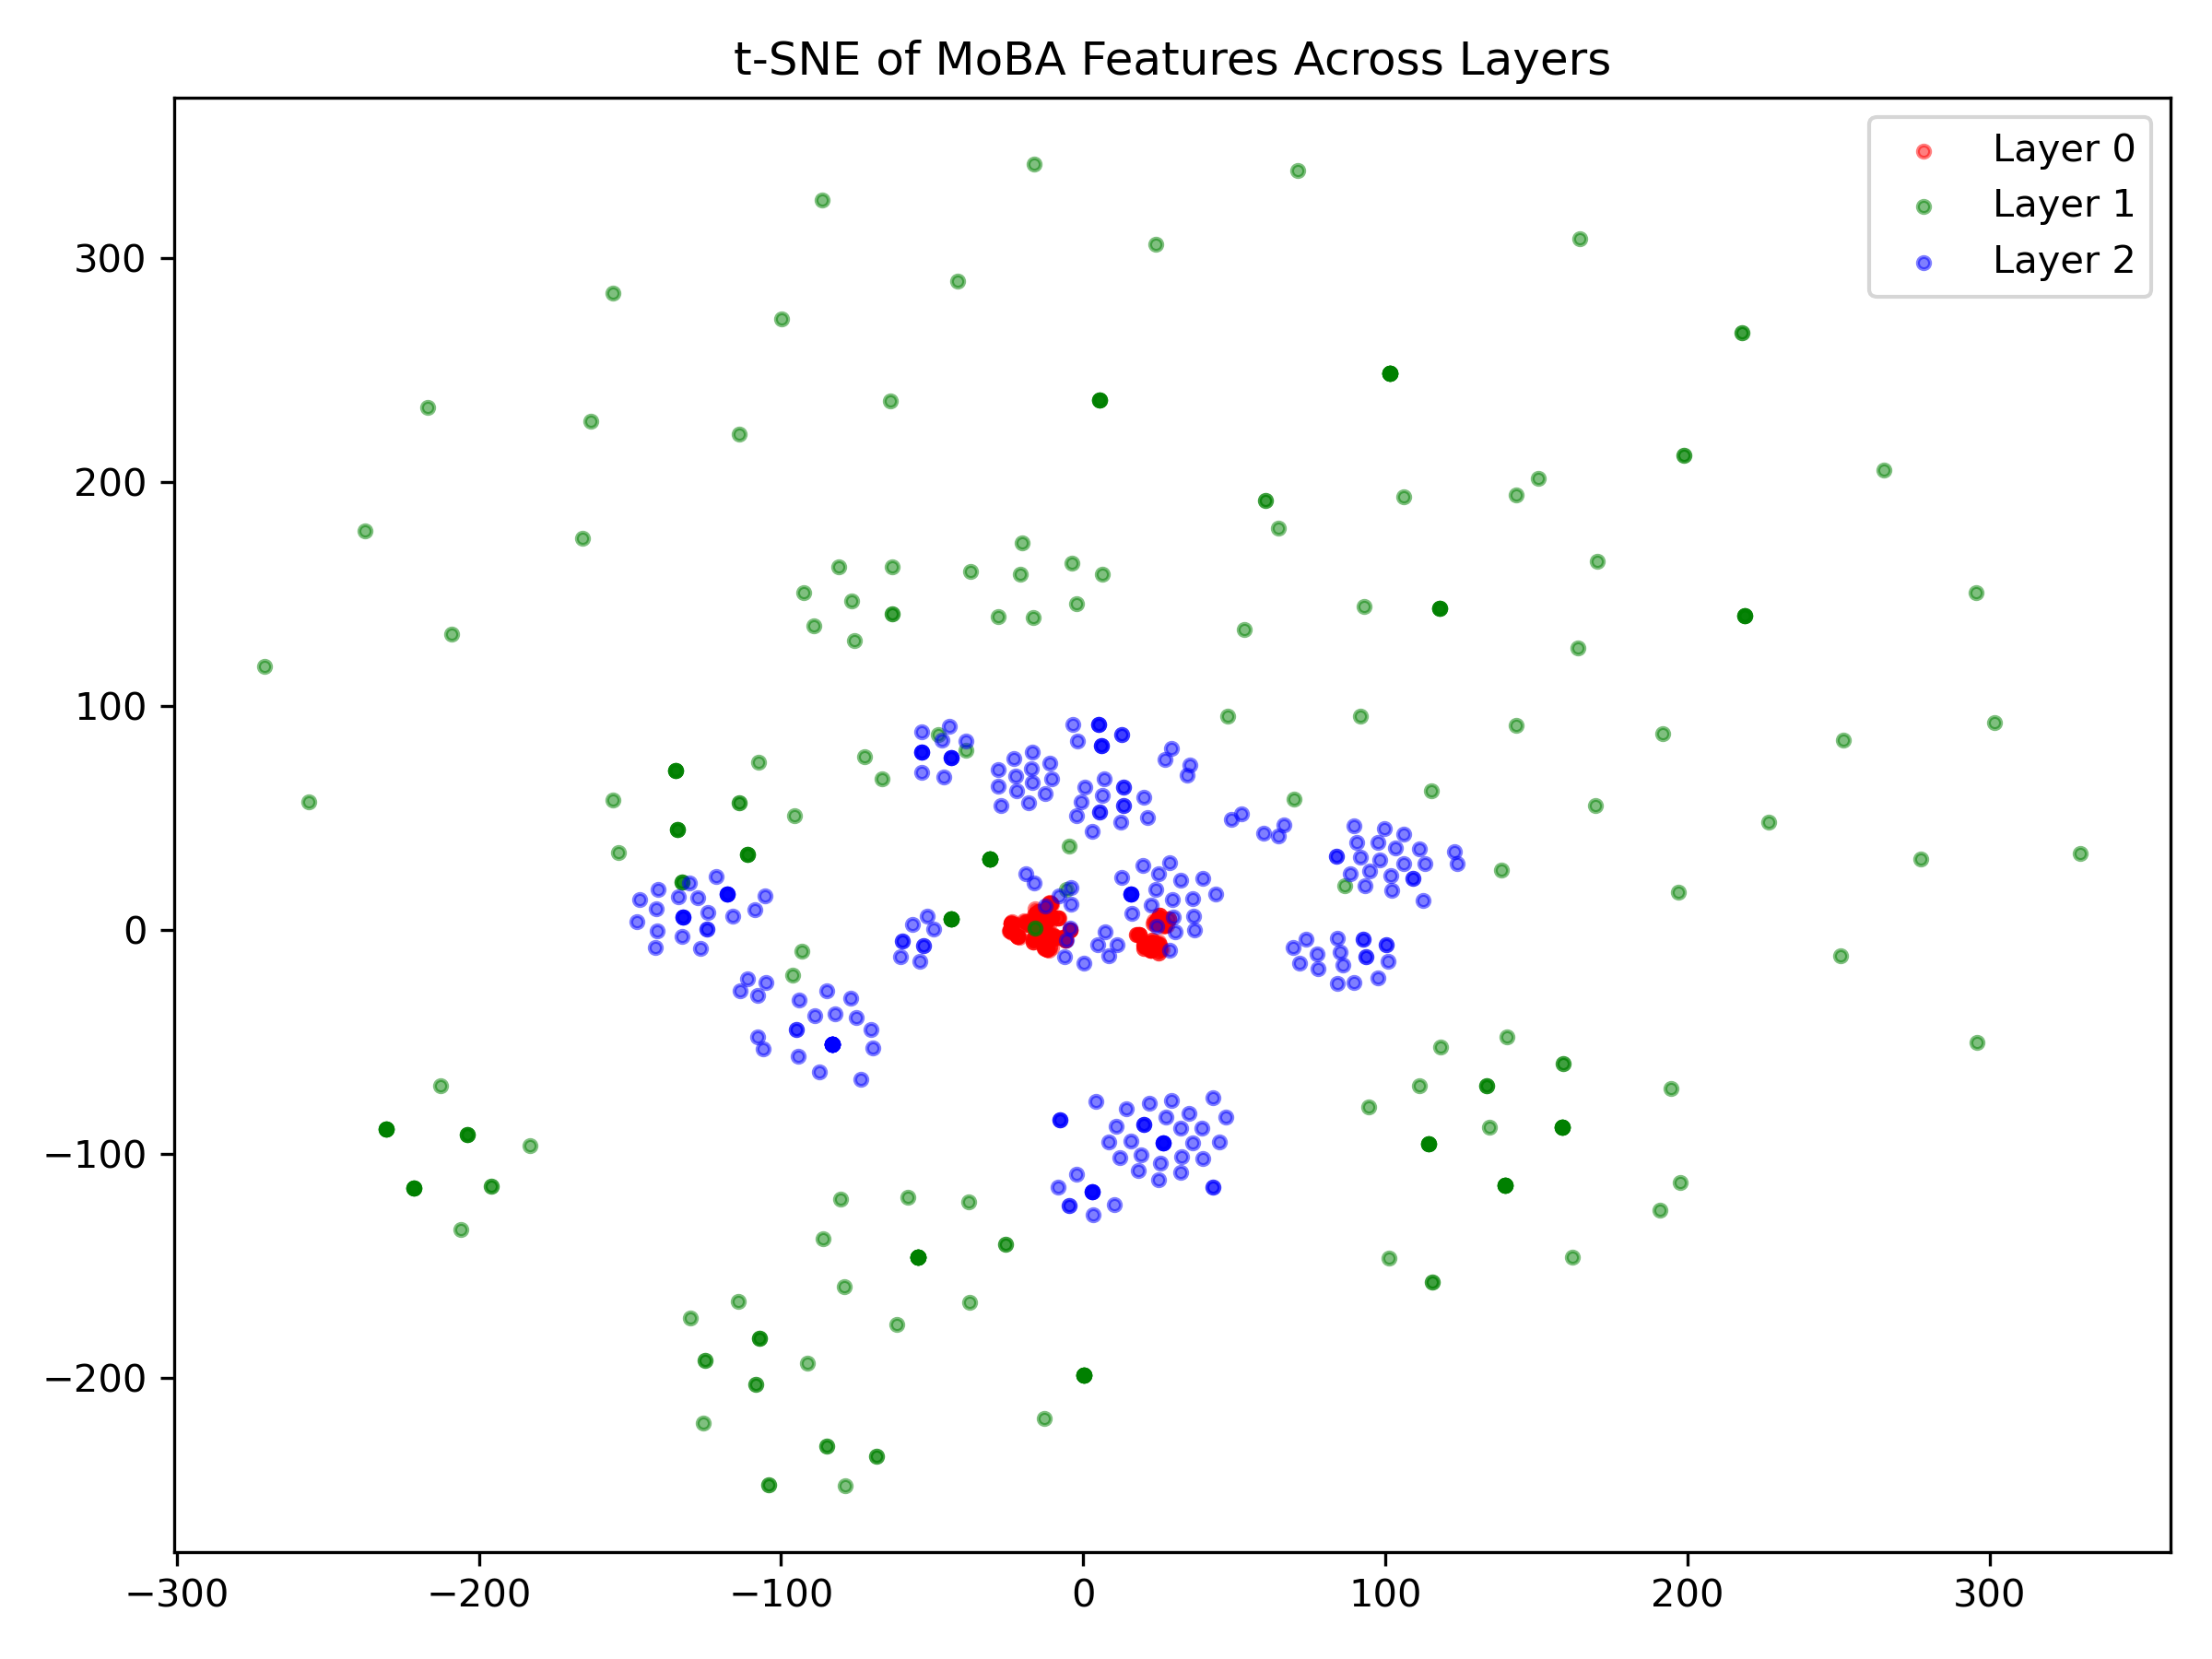
\includegraphics[width=0.8\textwidth]{7.png}  % ← 占全图
    \captionsetup{labelfont=bf,labelsep=space,font=small} % 全局可放导言区
    \caption{
      \textbf{The t-SNE visualization shows the distribution of inter node features from different layers  of the MoBA model in 2D space, highlighting how feature clustering and spatial distribution evolve across layers.} }
    \label{fig7}
\end{figure*}


 
\begin{figure*}[htbp]
    \centering
    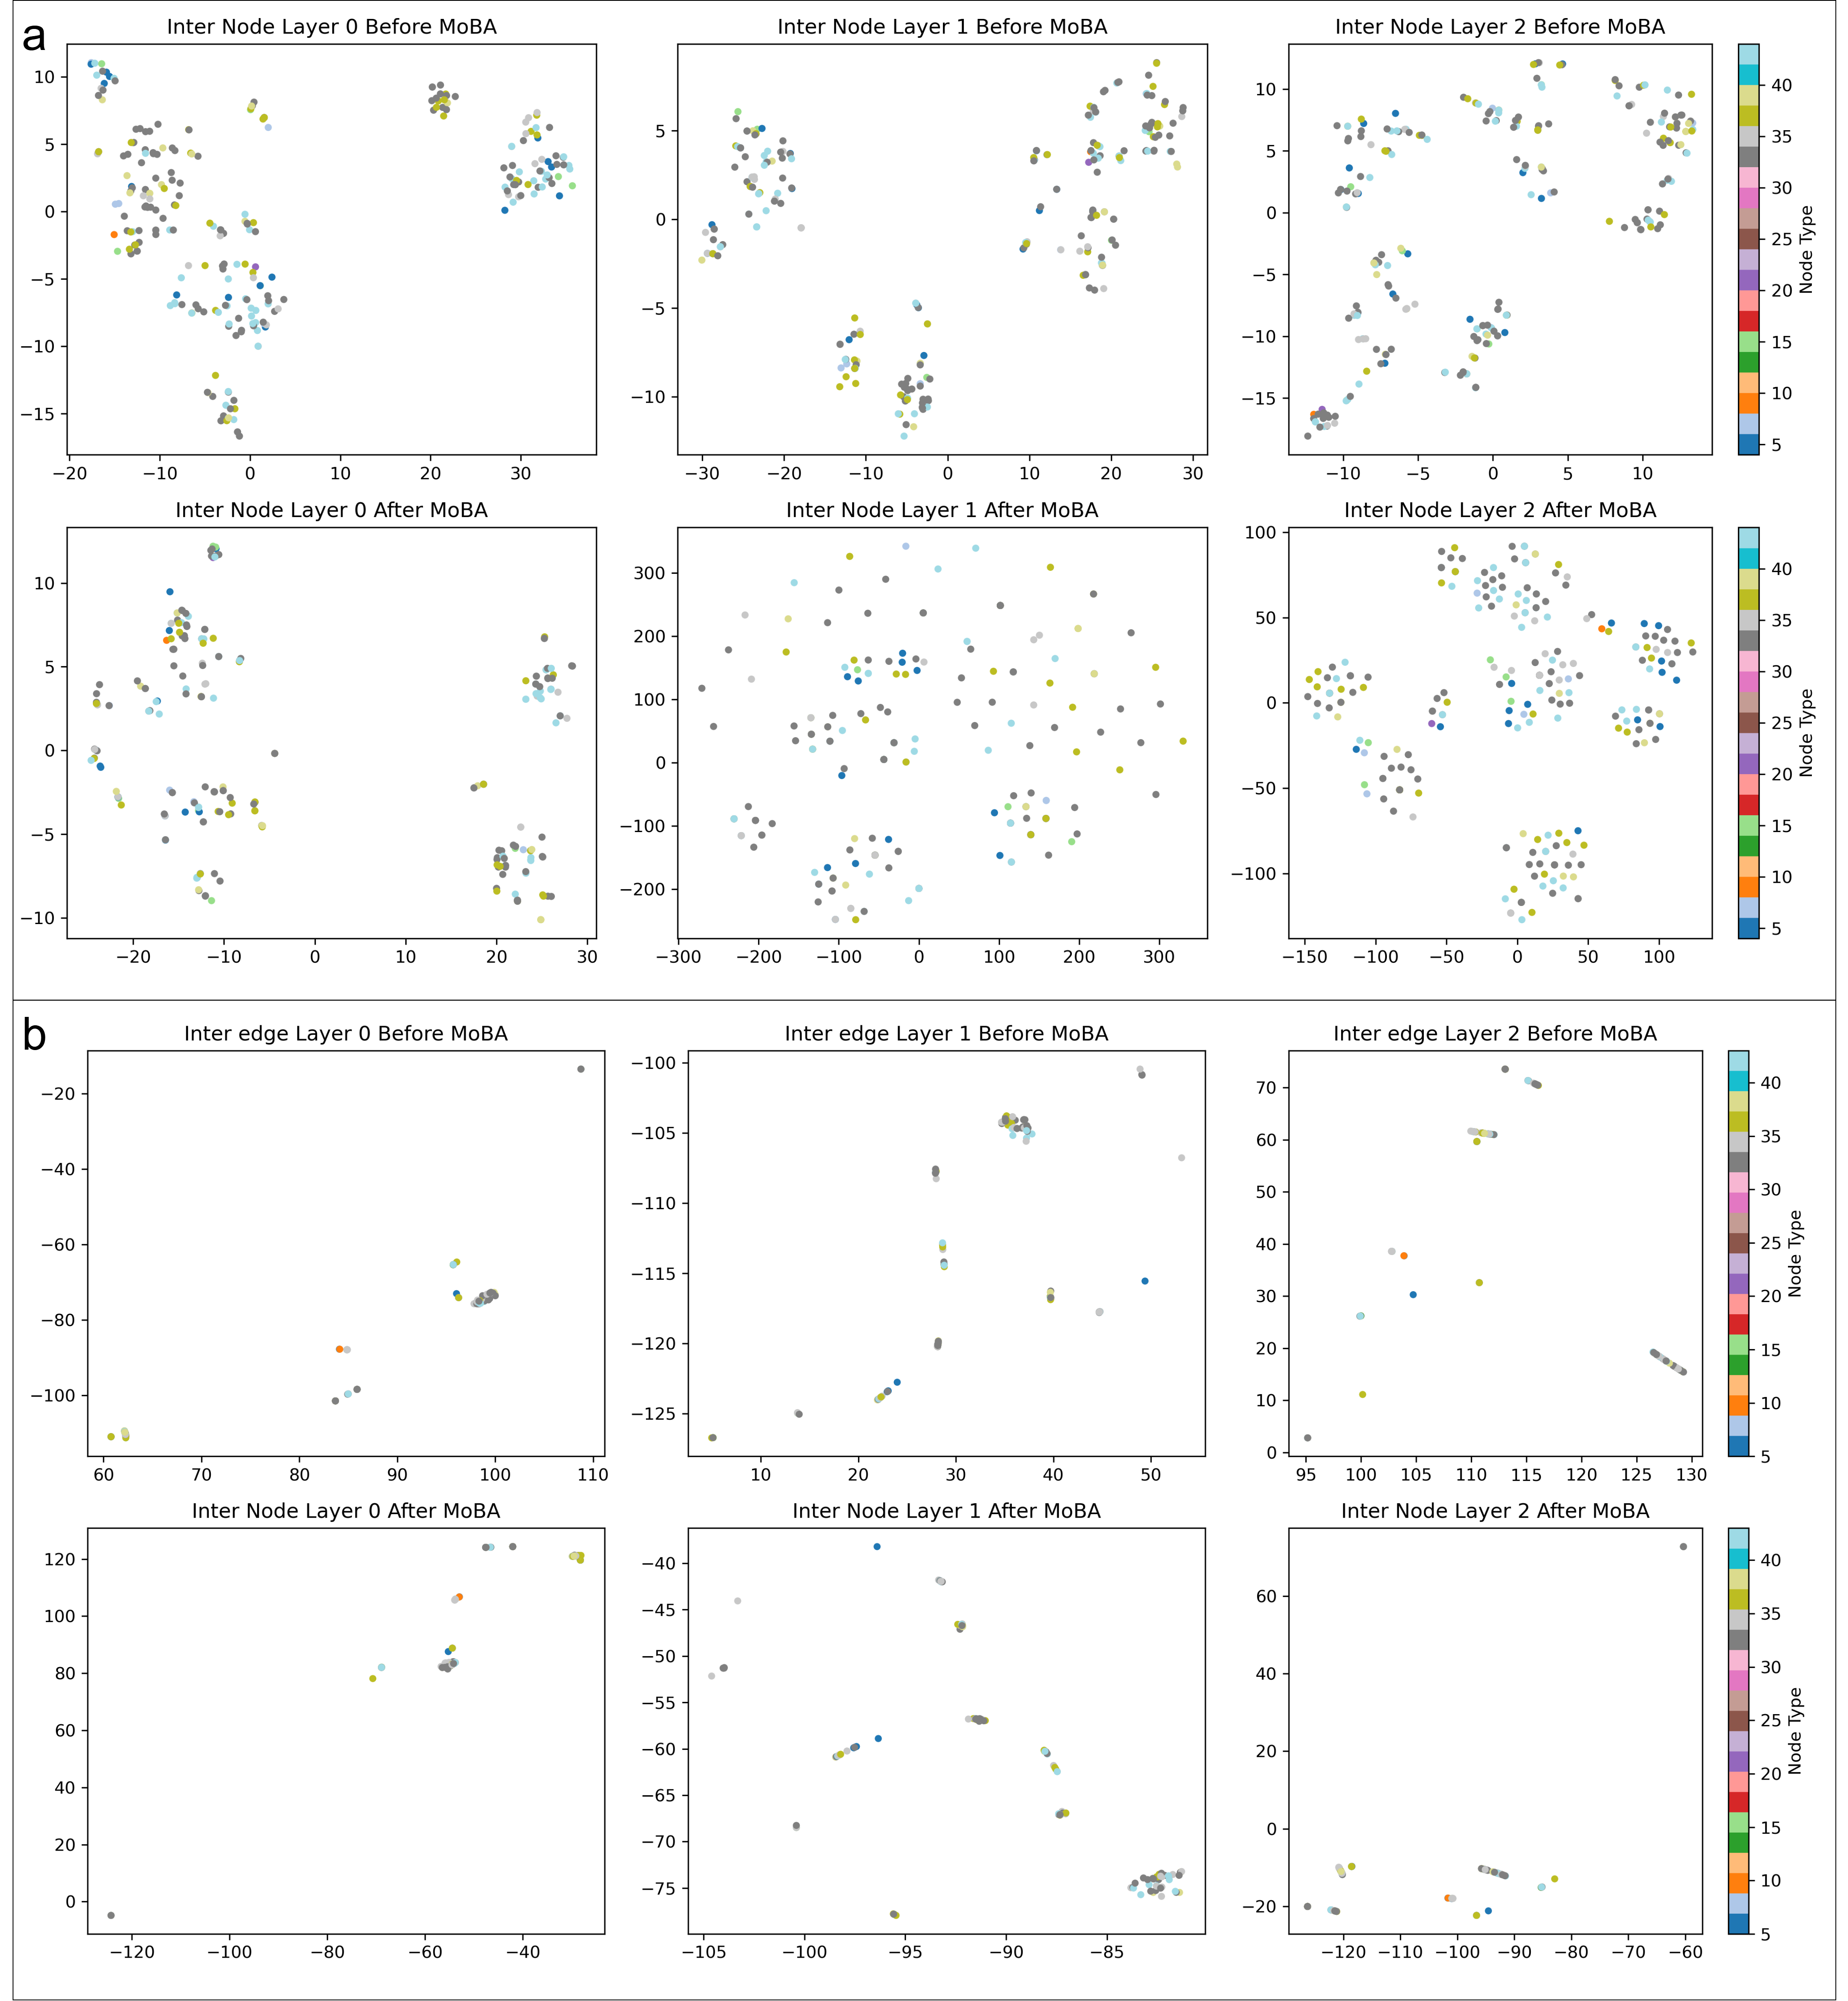
\includegraphics[width=1\textwidth]{8.png}  % ← 占全图
    \captionsetup{labelfont=bf,labelsep=space,font=small} % 全局可放导言区
    \caption{
      \textbf{Figure a presents the t-SNE visualizations of node features across different layers (0, 1, 2) before and after MoBA processing, while Figure b shows the corresponding edge features across the same layers. The color indicates node types, illustrating the impact of MoBA on the structural organization of node and edge feature spaces.} }
    \label{fig8}
\end{figure*}

 
\begin{figure*}[htbp]
    \centering
    \includegraphics[width=1\textwidth]{9.png}  % ← 占全图
    \captionsetup{labelfont=bf,labelsep=space,font=small} % 全局可放导言区
    \caption{
      \textbf{The t-SNE visualizations depict the distribution changes of both intra node features (Figure a) and intra edge features (Figure b) across various layers before and after applying MoBA. The colors represent different node types, allowing for a direct comparison of the clustering improvements and distribution differences of features due to MoBA processing at each layer.} }
    \label{fig9}
\end{figure*}

 
\begin{figure*}[htbp]
    \centering
    \includegraphics[width=1\textwidth]{10.png}  % ← 占全图
    \captionsetup{labelfont=bf,labelsep=space,font=small} % 全局可放导言区
    \caption{
      \textbf{This Figure presents the PCA-reduced distributions of inter node features (Figure a) and inter edge features (Figure b) across different layers before and after MoBA application. Colors represent node types, directly comparing the impact of MoBA on feature distribution and type separability for both node and edge features across layers.} }
    \label{fig10}
\end{figure*}

 
\begin{figure*}[htbp]
    \centering
    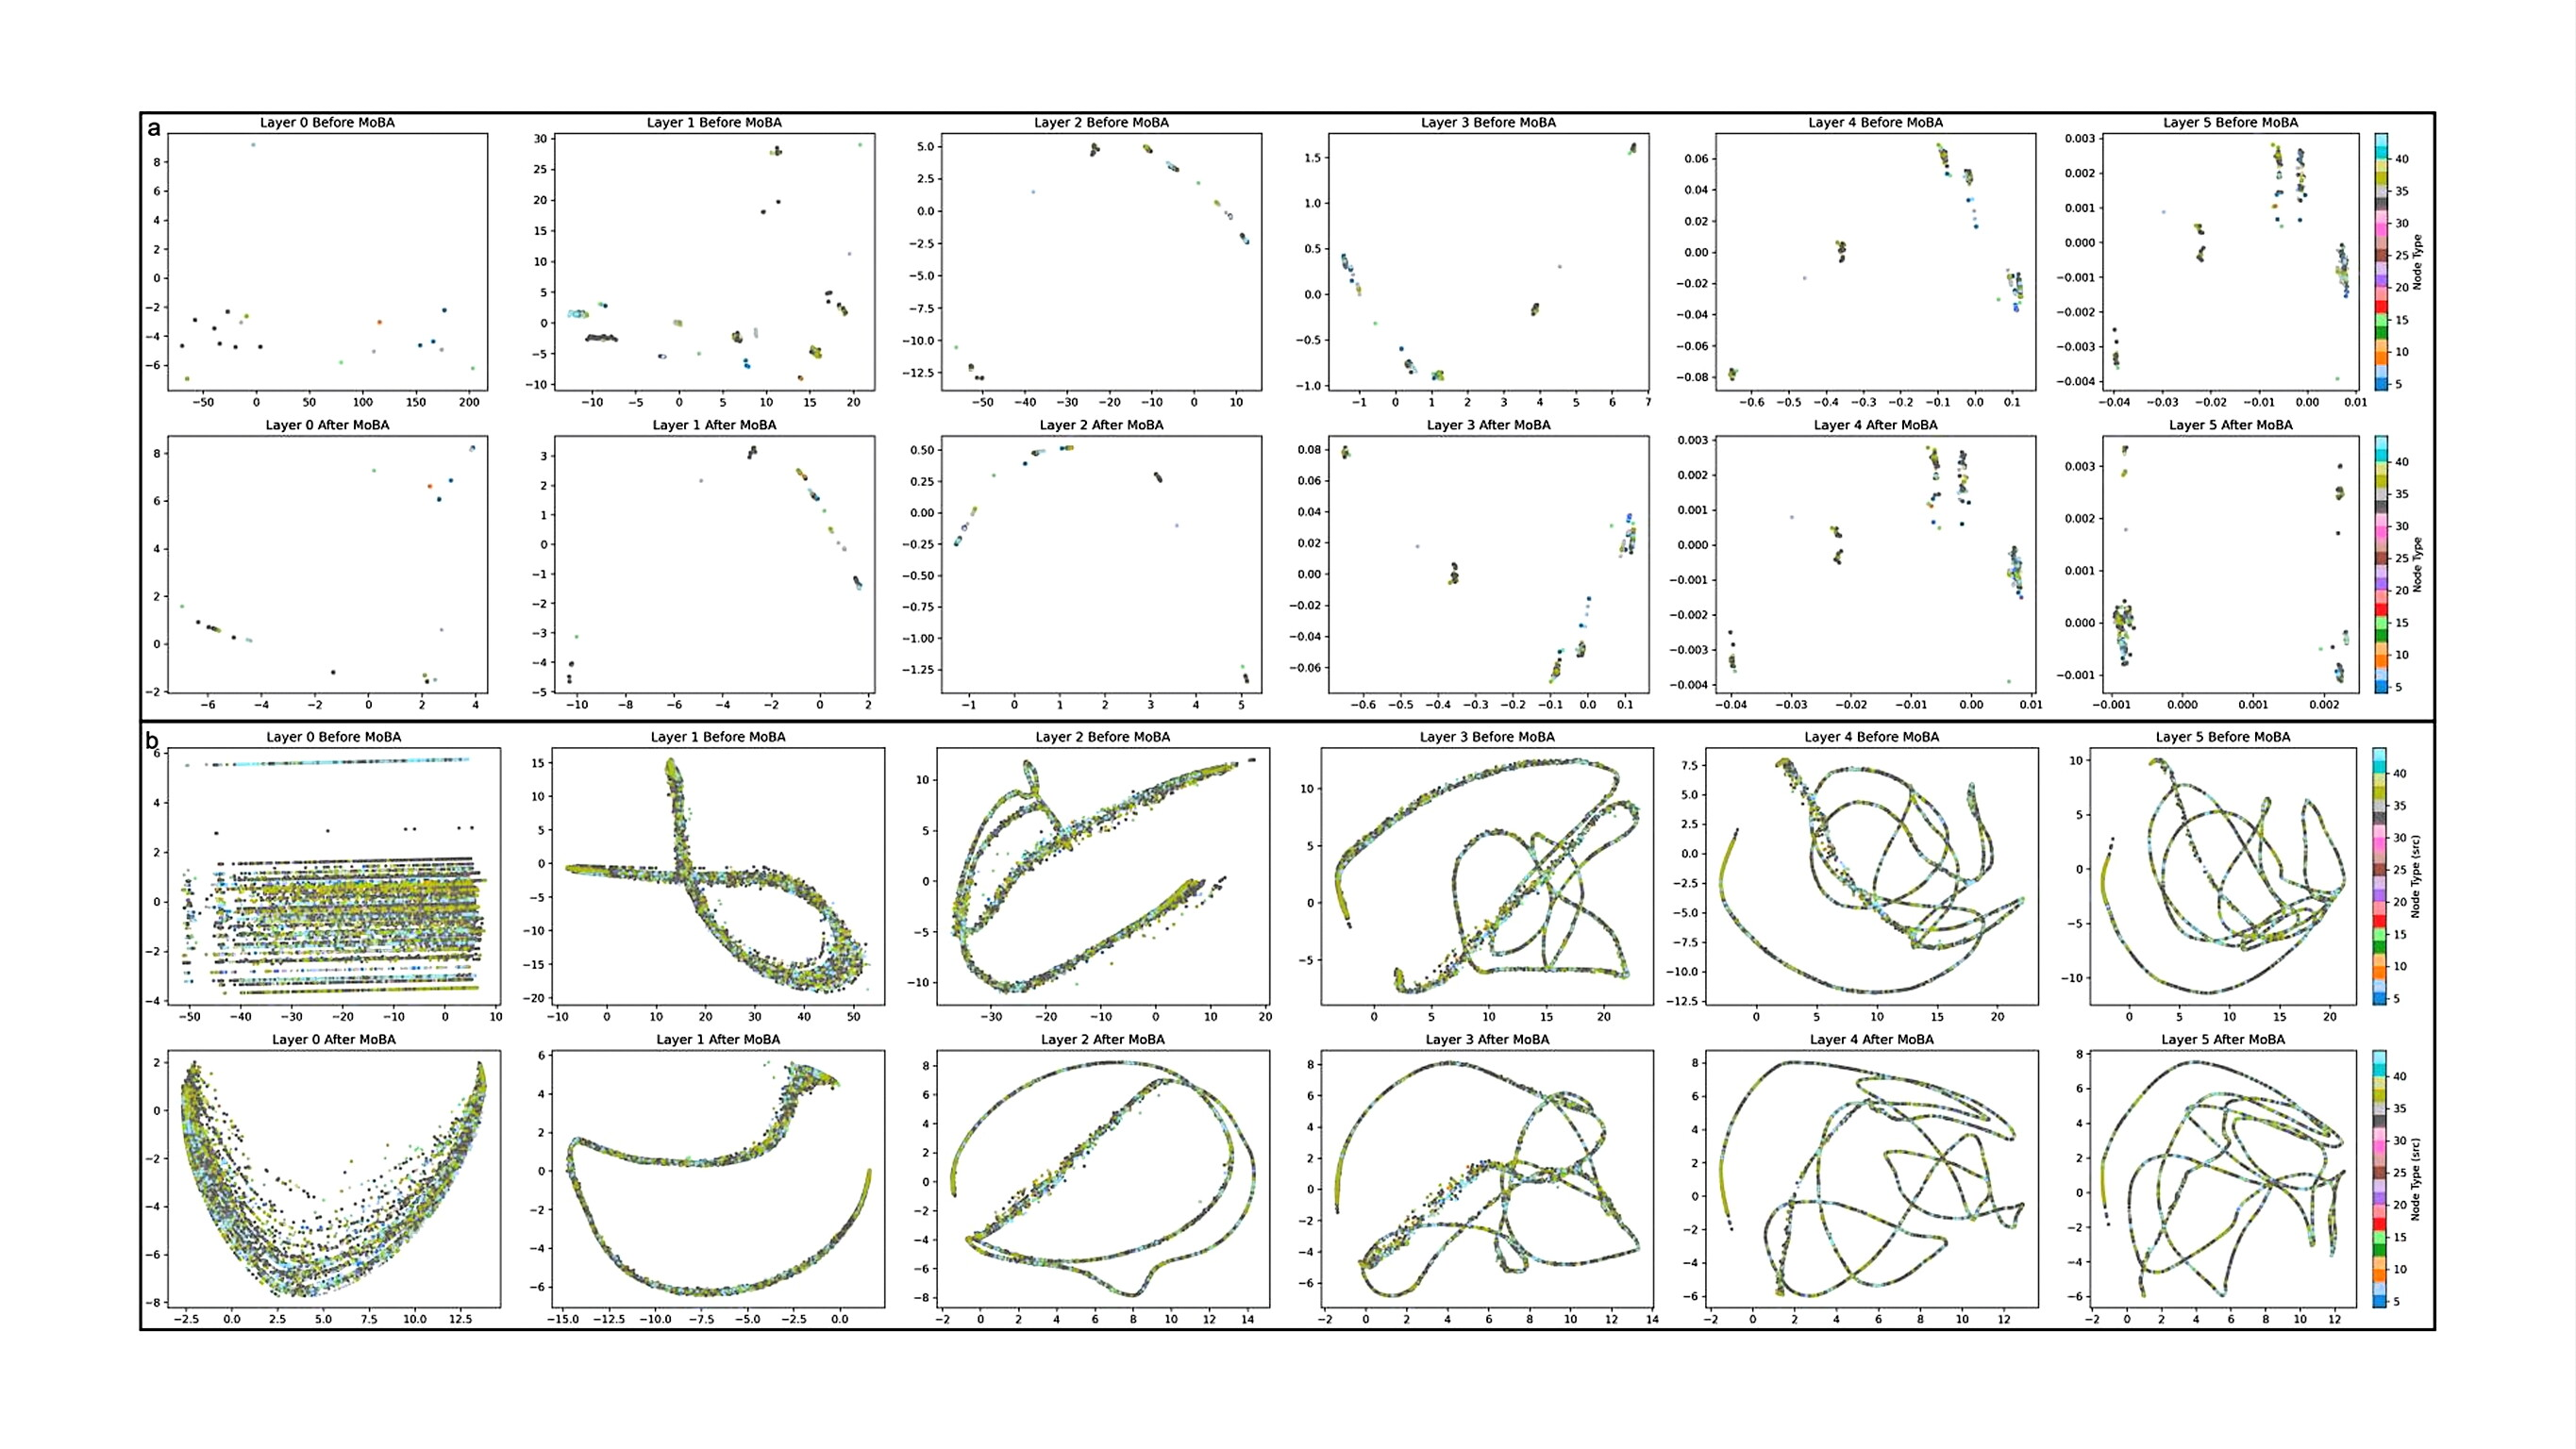
\includegraphics[width=1\textwidth]{11.png}  % ← 占全图
    \captionsetup{labelfont=bf,labelsep=space,font=small} % 全局可放导言区
    \caption{
      \textbf{This Figure illustrates the PCA-reduced distributions of intra node features (Figure a) and intra edge features (Figure b) across multiple layers before and after MoBA application. Colors denote node types, enabling a direct comparison of MoBA's impact on node feature distribution, type separability, and edge feature organization across different layers.} }
    \label{fig11}
\end{figure*}

 
\begin{figure*}[htbp]
    \centering
    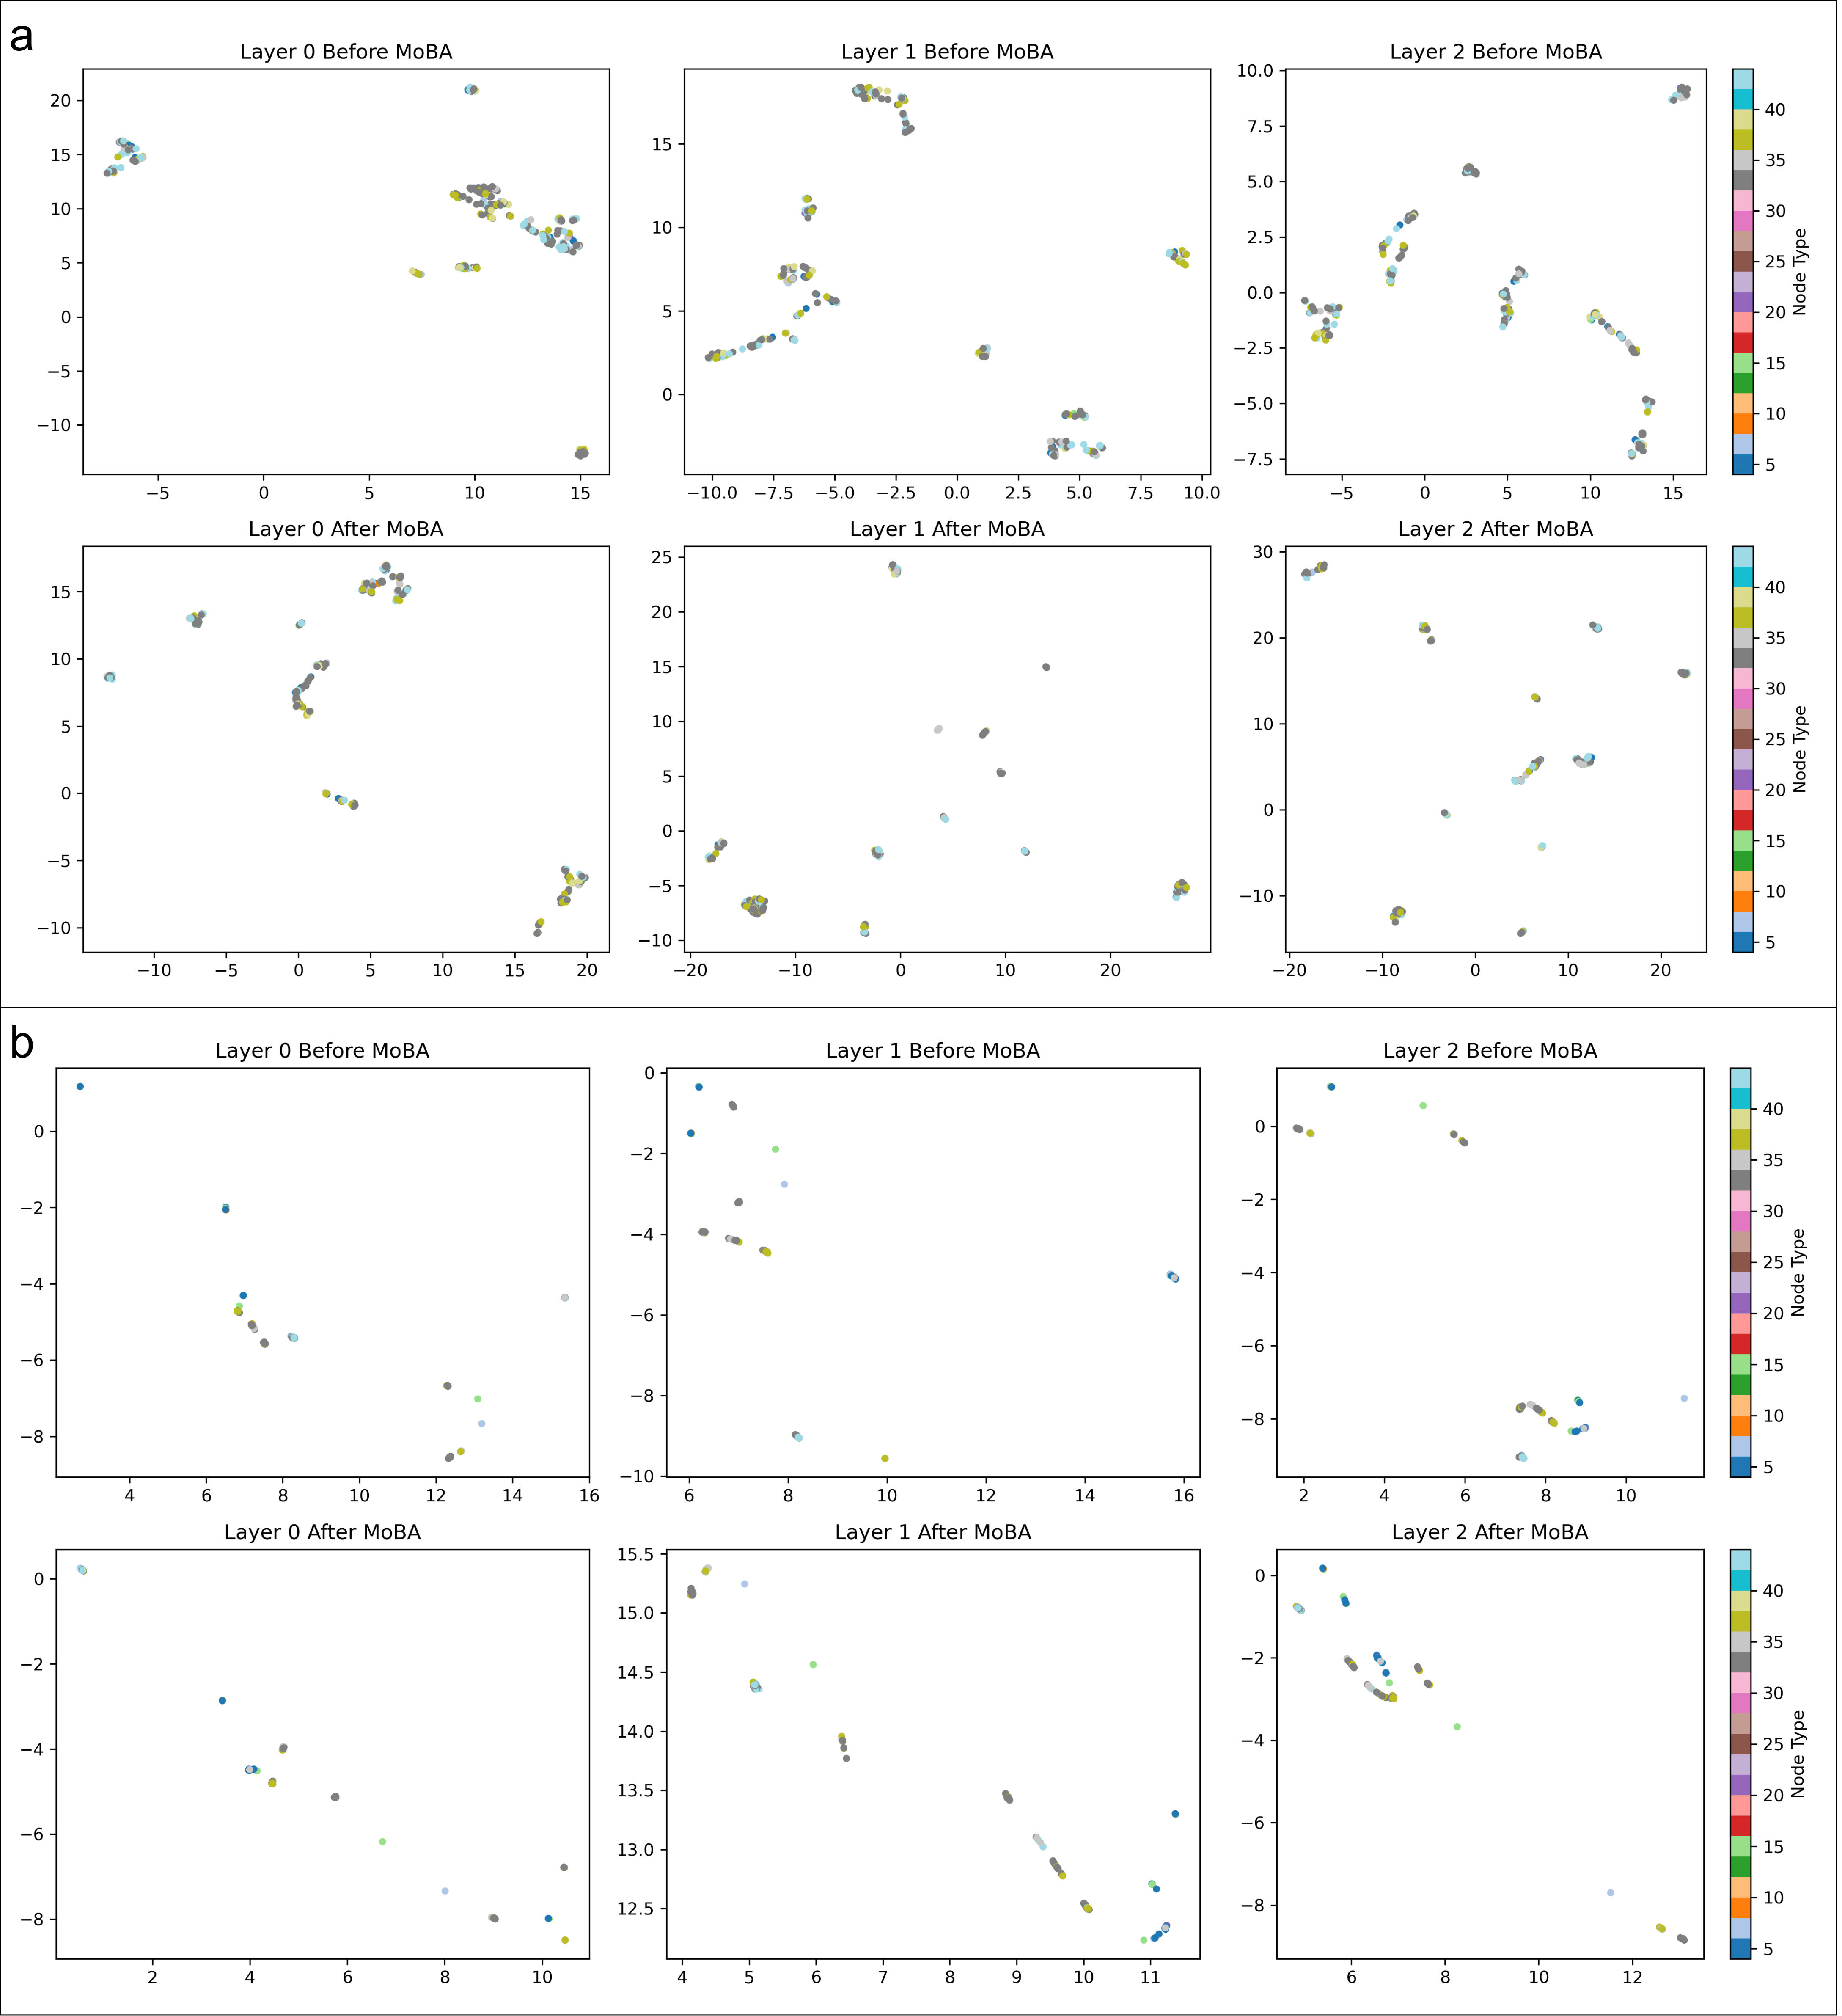
\includegraphics[width=1\textwidth]{12.png}  % ← 占全图
    \captionsetup{labelfont=bf,labelsep=space,font=small} % 全局可放导言区
    \caption{
      \textbf{The Figure illustrates the distribution changes of both inter node features (Figure a) and inter edge features (Figure b) across different layers before and after MoBA using UMAP. The visualizations directly compare the impact of MoBA on the clustering structure of node features, with colors indicating node types.} }
    \label{fig12}
\end{figure*}

 
\begin{figure*}[htbp]
    \centering
    \includegraphics[width=1\textwidth]{13.png}  % ← 占全图
    \captionsetup{labelfont=bf,labelsep=space,font=small} % 全局可放导言区
    \caption{
      \textbf{The Figure illustrates the distribution changes of both intra node features (Figure a) and intra edge features (Figure b) across different layers before and after MoBA using UMAP. It directly compares the impact of MoBA on the clustering structure of node features, with colors indicating node types.} }
    \label{fig13}
\end{figure*}

 
\begin{figure*}[htbp]
    \centering
    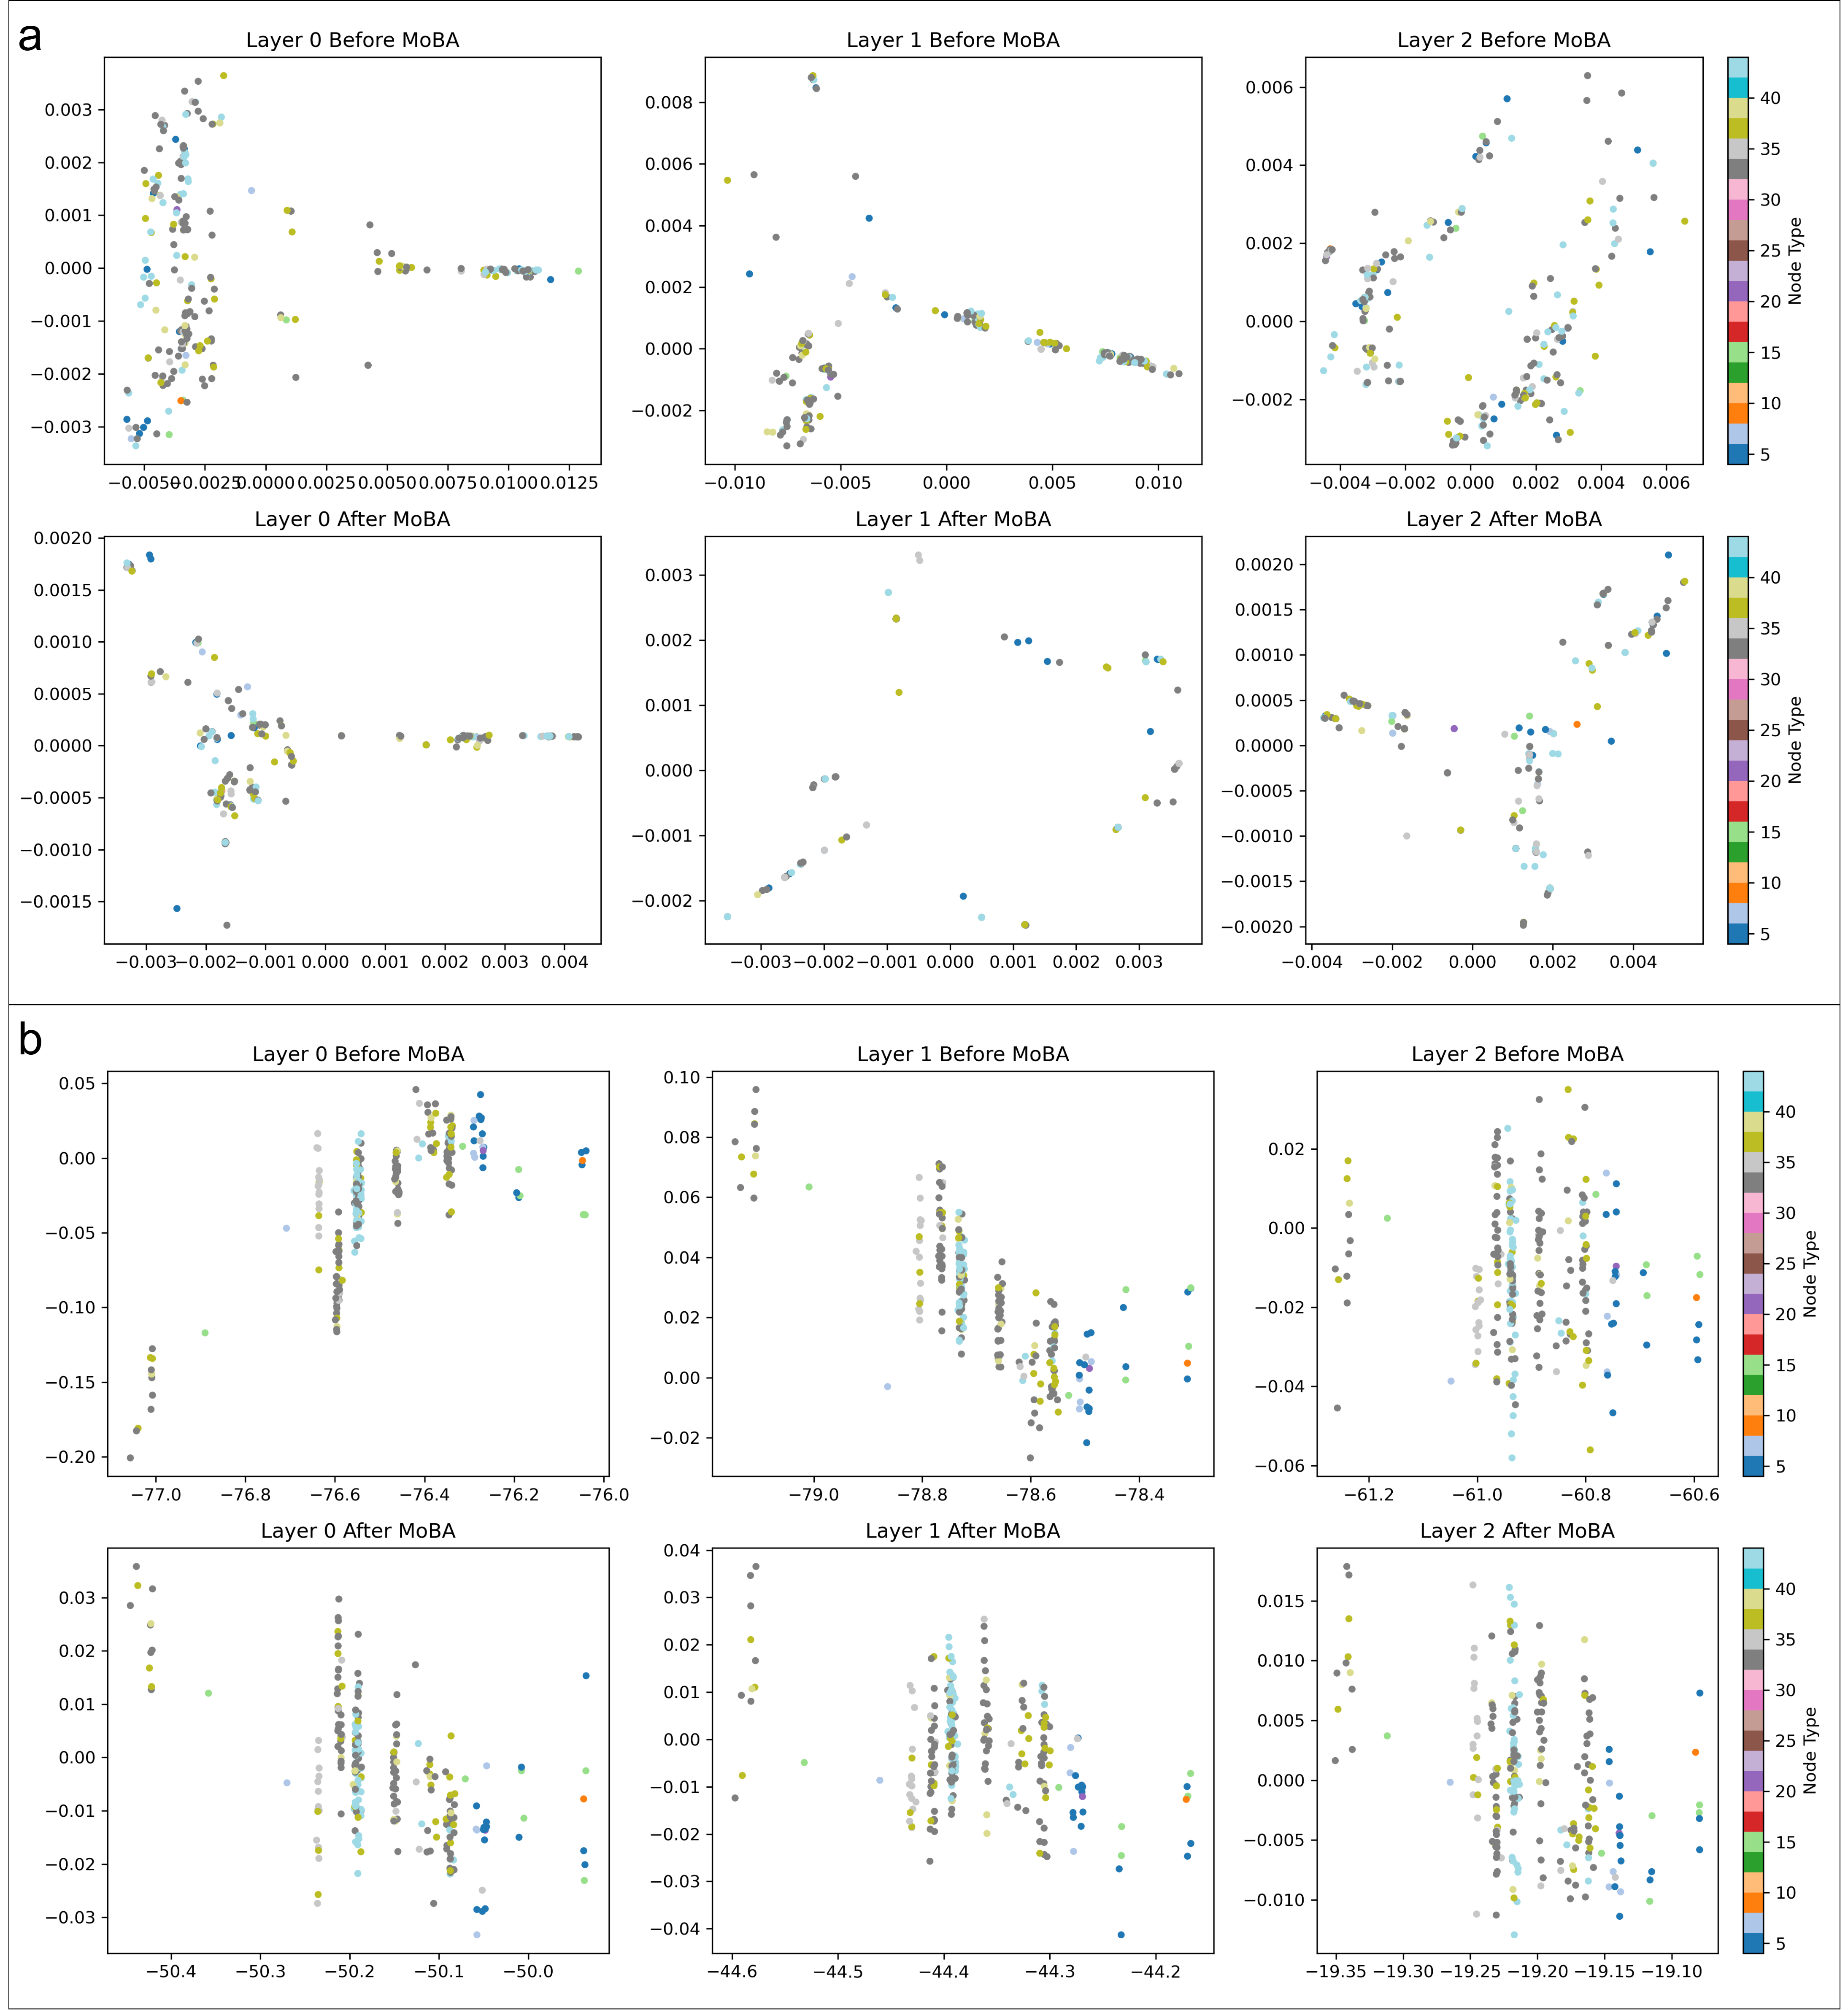
\includegraphics[width=1\textwidth]{14.png}  % ← 占全图
    \captionsetup{labelfont=bf,labelsep=space,font=small} % 全局可放导言区
    \caption{
      \textbf{The Figure presents Isomap projections of inter node features (Figure a) and inter edge features (Figure b) across different layers before and after MoBA, demonstrating the changes in feature space structure due to MoBA. Node types are indicated by colors, providing a visual comparison of feature distribution and clustering before and after MoBA application.} }
    \label{fig14}
\end{figure*}

 
\begin{figure*}[htbp]
    \centering
    \includegraphics[width=1\textwidth]{15.png}  % ← 占全图
    \captionsetup{labelfont=bf,labelsep=space,font=small} % 全局可放导言区
    \caption{
      \textbf{The Figure displays Isomap projections of both intra node features (Figure a) and intra edge features (Figure b) before and after MoBA across various layers, highlighting the changes in feature space structure induced by MoBA. Colors represent node types, providing a visual comparison of the feature distribution and clustering before and after MoBA application.} }
    \label{fig15}
\end{figure*}


\end{document}